%%%%%%%%%%%%%%%%%%%%%%%%%%%%%%%%%%%%%%%%%%%%%%%%%%%%%%%%%%%%%%%%%%%%%%%%%%%
%% This file is part of the book
%%
%% Algorithmic Graph Theory
%% http://code.google.com/p/graph-theory-algorithms-book/
%%
%% Copyright (C) 2010 David Joyner <wdjoyner@gmail.com>
%% Copyright (C) 2009--2011 Minh Van Nguyen <nguyenminh2@gmail.com>
%%
%% See the file COPYING for copying conditions.
%%%%%%%%%%%%%%%%%%%%%%%%%%%%%%%%%%%%%%%%%%%%%%%%%%%%%%%%%%%%%%%%%%%%%%%%%%%

\chapter{Introduction to Graph Theory}
\label{chap:introduction}

\begin{quote}
\footnotesize
\index{Eulerian trail}
\index{K\"onigsberg!seven bridges puzzle}
\index{treasure map}
\includegraphics[scale=0.7]{image/introduction/konigsberg-treasure-map} \\
\noindent
--- Spiked Math,
\url{http://spikedmath.com/120.html}
\end{quote}

\noindent
Our journey into graph theory starts with a puzzle that was solved
over 250 years ago by Leonhard
Euler~(1707--1783)\index{Euler!Leonhard}. The
Pregel\index{Pregel River} River flowed through the town of
K\"onigsberg\index{K\"onigsberg}, which is present day
Kaliningrad\index{Kaliningrad} in Russia\index{Russia}. Two islands
protruded from the river. On either side of the mainland, two bridges
joined one side of the mainland with one island and a third bridge
joined the same side of the mainland with the other island. A bridge
connected the two islands. In total, seven bridges connected the two
islands with both sides of the mainland. A popular exercise among the
citizens of K\"onigsberg\index{K\"onigsberg} was determining if it was
possible to cross each bridge exactly once during a single
walk\index{K\"onigsberg!seven bridges puzzle}. For historical
perspectives on this puzzle and Euler's\index{Euler!Leonhard}
solution, see\index{Gribkovskaia, Irina}\index{Halskau Sr., {\O}yvind}
Gribkovskaia\index{Laporte, Gilbert}~et~al.~\cite{GribkovskaiaEtAl2007}
and Hopkins\index{Hopkins, Brian} and
Wilson\index{Wilson, Robin}~\cite{HopkinsWilson2004}.

To visualize this puzzle in a slightly different way, consider
Figure~\ref{fig:introduction:seven_bridges_Konigsberg}. Imagine that
points $a$ and $c$ are either sides of the mainland, with points $b$
and $d$ being the two islands. Place the tip of your pencil on any of
the points $a,b,c,d$. Can you trace all the lines in the figure
exactly once, without lifting your pencil? Known as the seven bridges
of K\"onigsberg puzzle, Euler solved this problem in 1735 and with his
solution he laid the foundation of what is now known as graph theory.

\begin{figure}[!htbp]
\centering
\index{K\"onigsberg!graph}
\includegraphics{image/introduction/seven-bridges-Konigsberg}
\caption{The seven bridges of K\"onigsberg puzzle.}
\label{fig:introduction:seven_bridges_Konigsberg}
\end{figure}


%%%%%%%%%%%%%%%%%%%%%%%%%%%%%%%%%%%%%%%%%%%%%%%%%%%%%%%%%%%%%%%%%%%%%%%%%%%

\newpage

\section{Graphs and digraphs}
\label{sec:introduction:graphs_digraphs}

\begin{quote}
\footnotesize
When I use a word, it means just what I choose it to mean---neither
more nor less.\\
\noindent
--- Humpty Dumpty\index{Humpty Dumpty} in
Lewis Carroll's\index{Carroll, Lewis}
\emph{Through the Looking Glass}\index{Through the Looking Glass}
\end{quote}

\noindent
The word ``graph'' is commonly understood to mean a visual
representation of a dataset, such as a bar chart, a histogram, a
scatterplot, or a plot of a function. Examples of such graphs are
shown in Figure~\ref{fig:introduction:graphs_as_plots}.

\begin{figure}[!htbp]
\centering
\index{function plot}
\index{scatterplot}
\subfigure[Plots of functions.]{
  \includegraphics{image/introduction/graphs-as-plots-function.pdf}
}
\quad
\subfigure[A scatterplot.]{
  \includegraphics{image/introduction/graphs-as-plots-scatterplot.pdf}
}
\caption{Visual representations of datasets as plots.}
\label{fig:introduction:graphs_as_plots}
\end{figure}

This book is not about graphs in the sense of plots of functions or
datasets. Rather, our focus is on
\emph{combinatorial graphs}\index{combinatorial graphs} or
\emph{graphs} for short. A graph in the combinatorial sense is a
collection of discrete interconnected elements, an example of which is
shown in Figure~\ref{fig:introduction:seven_bridges_Konigsberg}. How
can we elaborate on this brief description of combinatorial graphs? To
paraphrase what Felix Klein\index{Klein, Felix} said about
curves,\footnote{
  ``Everyone knows what a curve is, until he has studied enough
  mathematics to become confused through the countless number of
  possible exceptions.''
}
it is easy to define a graph until we realize the countless number of
exceptions. There are directed graphs, weighted graphs, multigraphs,
simple graphs, and so on. Where do we begin?

\paragraph{Notation}
If $S$ is a set, let $S^{(n)}$ denote the set of unordered
$n$-tuples\index{tuple}~(with possible repetition). We shall sometimes
refer to an unordered $n$-tuple as an
\emph{$n$-set}\index{set!$n$-set}. \\

\noindent
We start by calling a ``graph'' what some call an
``unweighted\index{graph!unweighted},
undirected\index{graph!undirected} graph without
multiple\index{edge!multiple} edges.''

\begin{definition}
\rm
A \emph{graph}\index{graph} $G = (V, E)$ is an ordered pair of finite
sets. Elements of $V$ are called \emph{vertices}\index{vertex} or
\emph{nodes}\index{node}, and elements of $E \subseteq V^{(2)}$ are
called \emph{edges}\index{edge} or \emph{arcs}\index{arcs}. We refer
to $V$ as the \emph{vertex set}\index{vertex!set} of $G$, with $E$
being the \emph{edge set}\index{edge!}. The cardinality of $V$ is
called the \emph{order}\index{order} of $G$, and $|E|$ is called the
\emph{size}\index{size} of $G$. We usually disregard any direction of
the edges and consider $(u,v)$ and $(v,u)$ as one and the same edge in
$G$. In that case, $G$ is referred to as an
\emph{undirected graph}\index{graph!undirected}.
\end{definition}

One can label a graph by attaching labels to its vertices.
If $(v_1, v_2) \in E$ is an edge of a graph $G = (V, E)$, we say that
$v_1$ and $v_2$ are \emph{adjacent}\index{vertex!adjacent}
vertices. For ease of notation, we write the edge $(v_1, v_2)$ as
$v_1 v_2$. The edge $v_1 v_2$ is also said to be
\emph{incident}\index{edge!incident} with the vertices $v_1$ and
$v_2$.

\begin{figure}[!htbp]
\centering
\index{house graph}
\includegraphics{image/introduction/house-graph}
\caption{A house graph.}
\label{fig:introduction:house_graph}
\end{figure}

\begin{example}
\label{eg:introduction:house_graph}
Consider the graph in Figure~\ref{fig:introduction:house_graph}.
%%
\begin{enumerate}
\item List the vertex and edge sets of the graph.

\item For each vertex, list all vertices that are adjacent to it.

\item Which vertex or vertices have the largest number of adjacent
  vertices? Similarly, which vertex or vertices have the smallest
  number of adjacent vertices?

\item If all edges of the graph are removed, is the resulting figure
  still a graph? Why or why not?

\item If all vertices of the graph are removed, is the resulting
  figure still a graph? Why or why not?
\end{enumerate}
\end{example}

\begin{proof}[Solution]
(1)~Let $G = (V, E)$ denote the graph in
Figure~\ref{fig:introduction:house_graph}. Then the vertex set of $G$
is $V = \{ a, b, c, d, e \}$. The edge set of $G$ is given by
%%
\begin{equation}
\label{eqn:introduction:edges_of_house_graph}
E
=
\{ab,\, ae,\, ba,\, bc,\, be,\, cb,\, cd,\, dc,\, de,\, ed,\, eb,\, ea\}.
\end{equation}
%%
We can also use Sage to construct the graph $G$ and list its vertex
and edge sets:
%%
\begin{lstlisting}
sage: G = Graph({"a":["b","e"], "b":["a","c","e"], "c":["b","d"],
...   "d":["c","e"], "e":["a","b","d"]})
sage: G
Graph on 5 vertices
sage: G.vertices()
['a', 'b', 'c', 'd', 'e']
sage: G.edges(labels=False)
[('a', 'b'), ('a', 'e'), ('b', 'e'), ('c', 'b'), ('c', 'd'), ('e', 'd')]
\end{lstlisting}
%%
The graph $G$ is undirected, meaning that we do not impose direction
on any edges. Without any direction on the edges, the edge $ab$ is the
same as the edge $ba$. That is why \texttt{G.edges()} returns six
edges instead of the 12 edges listed
in~\eqref{eqn:introduction:edges_of_house_graph}.

(2)~Let $\adj(v)$\index{$\adj$} be the set of all vertices that are
adjacent to $v$. Then we have
%%
\begin{align*}
\text{adj}(a) &= \{ b, e \} \\
\text{adj}(b) &= \{ a, c, e \} \\
\text{adj}(c) &= \{ b, d \} \\
\text{adj}(d) &= \{ c, e \} \\
\text{adj}(e) &= \{ a, b, d \}.
\end{align*}
%%
The vertices adjacent to $v$ are also referred to as its
\emph{neighbors}. We can use the function \texttt{G.neighbors()} to
list all the neighbors of each vertex.
%%
\begin{lstlisting}
sage: G.neighbors("a")
['b', 'e']
sage: G.neighbors("b")
['a', 'c', 'e']
sage: G.neighbors("c")
['b', 'd']
sage: G.neighbors("d")
['c', 'e']
sage: G.neighbors("e")
['a', 'b', 'd']
\end{lstlisting}

(3)~Taking the cardinalities of the above five sets, we get
$|\text{adj}(a)| = |\text{adj}(c)| = |\text{adj}(d)| = 2$ and
$|\text{adj}(b)| = |\text{adj}(e)| = 3$. Thus $a$, $c$ and $d$ have
the smallest number of adjacent vertices, while $b$ and $e$ have the
largest number of adjacent vertices.

(4)~If all the edges in $G$ are removed, the result is still a graph,
although one without any edges. By definition, the edge set of any
graph is a subset of $V^{(2)}$. Removing all edges of $G$ leaves us
with the empty set $\emptyset$, which is a subset of every set.

(5)~Say we remove all of the vertices from the graph in
Figure~\ref{fig:introduction:house_graph} and in the process all edges
are removed as well. The result is that both of the vertex and edge
sets are empty. This is a special graph known as the \emph{empty} or
\emph{null}\index{null graph} graph.
\end{proof}

\begin{example}
Consider the illustration in
Figure~\ref{fig:introduction:self_loop}. Does
Figure~\ref{fig:introduction:self_loop} represent a graph? Why or why
not?
\end{example}

\begin{proof}[Solution]
If $V = \{ a, b, c \}$ and $E = \{ aa, bc \}$, it is clear that $E
\subseteq V^{(2)}$. Then $(V, E)$ is a graph. The edge $aa$ is
called a \emph{self-loop}\index{self-loop} of the graph. In general,
any edge of the form $vv$ is a self-loop.
\end{proof}

\begin{figure}[!htbp]
\centering
\includegraphics{image/introduction/self-loop}
\caption{A figure with a self-loop.}
\label{fig:introduction:self_loop}
\end{figure}

In Figure~\ref{fig:introduction:house_graph}, the edges $ae$ and $ea$
represent one and the same edge. If we do not consider the direction
of the edges in the graph of
Figure~\ref{fig:introduction:house_graph}, then the graph has six
edges. However, if the direction of each edge is taken into account,
then there are 12 edges as listed
in~\eqref{eqn:introduction:edges_of_house_graph}. The following
definition captures the situation where the direction of the edges are
taken into account.

A \emph{directed edge}\index{edge!directed} is an edge such that one
vertex incident with it is designated as the
\emph{head}\index{vertex!head} vertex and the other incident vertex is
designated as the \emph{tail}\index{vertex!tail} vertex. In this
situation, we may assume that the set of edges is a subset of the
ordered pairs $V \times V$. A directed edge $uv$ is said to be
directed from its tail $u$ to its head $v$. A
\emph{directed graph}\index{graph!directed} or
\emph{digraph}\index{digraph} $G$ is a graph each of whose edges is
directed. The \emph{indegree}\index{indegree} $\id(v)$\index{$\id$} of
a vertex $v \in V(G)$ counts the number of edges such that $v$ is the
head of those edges. The \emph{outdegree}\index{outdegree}
$\od(v)$\index{$\od$} of a vertex $v \in V(G)$ is the number of edges
such that $v$ is the tail of those edges. The
\emph{degree}\index{degree} $\deg(v)$\index{$\deg$} of a vertex $v$ of
a digraph is the sum of the indegree and the outdegree of $v$.

Let $G$ be a graph without self-loops and multiple edges. It is
important to distinguish a graph $G$ as being directed or undirected.
If $G$ is undirected and $uv \in E(G)$, then $uv$ and $vu$
represent the same edge. In case $G$ is a digraph, then $uv$ and $vu$
are different directed edges. For a digraph $G = (V, E)$ and a vertex
$v \in V$, all the neighbors of $v$ in $G$ are contained in $\adj(v)$,
i.e. the set of all neighbors of $v$. Just as we distinguish between
indegree and outdegree for a vertex in a digraph, we also distinguish
between in-neighbors and out-neighbors. The set of
\emph{in-neighbors}\index{in-neighbor}
$\iadj(v) \subseteq \adj(v)$\index{$\iadj$} of $v \in V$ consists of
all those vertices that contribute to the indegree of $v$. Similarly,
the set of \emph{out-neighbors}\index{out-neighbor}
$\oadj(v) \subseteq \adj(v)$\index{$\oadj$} of $v \in V$ are those
vertices that contribute to the outdegree of $v$. Then
\[
\iadj(v) \cap \oadj(v)
=
\{u \mid uv \in E \text{ and } vu \in E\}
\]
and $\adj(v) = \iadj(v) \cup \oadj(v)$.


%%%%%%%%%%%%%%%%%%%%%%%%%%%%%%%%%%%%%%%%%%%%%%%%%%%%%%%%%%%%%%%%%%%%%%%%%%%

\subsection{Multigraphs}

This subsection presents a larger class of graphs. For simplicity of
presentation, in this book we shall assume \emph{usually} that a graph
is not a multigraph. In other words, when you read a property of
graphs later in the book, it will be assumed~(unless stated explicitly
otherwise) that the graph is not a multigraph. However, as multigraphs
and weighted graphs \emph{are} very important in many applications, we
will try to keep them in the back of our mind. When appropriate, we
will add as a remark how an interesting property of ``ordinary''
graphs extends to the multigraph or weighted graph case.

An important class of graphs consist of those graphs having multiple
edges between pairs of vertices. A \emph{multigraph}\index{multigraph}
is a graph in which there are multiple edges between a pair of
vertices. A \emph{multi-undirected graph}\index{multi-undirected graph}
is a multigraph that is undirected. Similarly, a
\emph{multidigraph}\index{multidigraph} is a directed multigraph.

\begin{example}
\rm
Sage can compute with and plot multigraphs, or multidigraphs, having
loops.
%%
\begin{lstlisting}
sage: G = Graph({0:{0:'e0',1:'e1',2:'e2',3:'e3'}, 2:{5:'e4'}})
sage: G.show(vertex_labels=True, edge_labels=True, graph_border=True)
sage: H = DiGraph({0:{0:"e0"}}, Loops=True)
sage: H.add_edges([(0,1,'e1'), (0,2,'e2'), (0,2,'e3'), (1,2,'e4'), (1,0,'e5')])
sage: H.show(vertex_labels=True, edge_labels=True, graph_border=True)
\end{lstlisting}
%%
These graphs are plotted in Figure~\ref{fig:introduction:graph_digraph}.

\begin{figure}[!htbp]
\centering
\subfigure[]{
  \includegraphics{image/introduction/graph-digraph_graph}
}
\qquad
\subfigure[]{
  \includegraphics{image/introduction/graph-digraph_digraph}
}
\caption{A graph $G$ and digraph $H$ with a loop and multi-edges.}
\label{fig:introduction:graph_digraph}
\end{figure}
\end{example}


As we indicated above, a graph may have ``weighted''\index{edge!weight}
edges.

\begin{definition}
\rm
A \emph{weighted graph}\index{graph!weighted} is a graph $G = (V, E)$
where each set $V$ and $E$ is a pair consisting of a vertex and a real
number called the \emph{weight}\index{weight!graph}.
\end{definition}

The illustration in
Figure~\ref{fig:introduction:seven_bridges_Konigsberg} is actually a
multigraph, a graph with multiple edges, called the
K\"onigsberg\index{K\"onigsberg!graph} graph.

\begin{definition}
\label{def:introduction:graph-version3}
\rm
For a weighted multigraph\index{weight!multigraph} $G$, we are
given:
%%
\begin{itemize}
\item A finite set $V$ whose elements are pairs $(v, w_v)$, where $v$
  is called a \emph{vertex}\index{vertex!multigraph} and $w_v \in \R$
  is called its \emph{weight}\index{weight!multigraph}. (Sometimes,
  the pair $(v, w_v)$ is called the vertex.)

\item A finite set $E$ whose elements are called
  \emph{edges}\index{edge!multigraph}. We do not necessarily assume
  that $E \subseteq V^{(2)}$, where $V^{(2)}$ is the set of unordered
  pairs of
  vertices.\footnote{
    However, we always assume that $E \subseteq \R \times V^{(2)}$,
    where the $\R$-component is called the
    \emph{weight}\index{edge!weight} of the edge.
  }

\item An incidence\index{incidence!function} function
%%
\begin{equation}
\label{eqn:introduction:edge_incidence}
i: E \to V^{(2)}.
\end{equation}
\end{itemize}
%%
Such a multigraph is denoted $G = (V,E,i)$. An
\emph{orientation}\index{orientation} on $G$ is a function
%%
\begin{equation}
\label{eqn:introduction:edge_orientation}
h: E \to V
\end{equation}
%%
where $h(e) \in i(e)$ for all $e \in E$. The element $v = h(e)$ is
called the \emph{head}\index{edge!head} of $i(e)$. If $G$ has no
self-loops, then $i(e)$ is a set having exactly two elements denoted
$i(e) = \{h(e),\, t(e)\}$. The element $v = t(e)$ is called the
\emph{tail}\index{edge!tail} of $i(e)$. For self-loops, we set
$t(e) = h(e)$. A multigraph with an orientation\index{orientation} can
therefore be described as the $4$-tuple $(V, E, i, h)$. In other
words, $G = (V,E,i,h)$ is a multidigraph.
Figure~\ref{fig:introduction:weighted_multigraph} illustrates a
weighted multigraph.
\end{definition}

\begin{figure}[!htbp]
\centering
\includegraphics{image/introduction/weighted-multigraph}
\caption{An example of a weighted multigraph.}
\label{fig:introduction:weighted_multigraph}
\end{figure}
%% sage: M = matrix([[0,1,3,0,6],[0,0,1,3,0],[1,2,0,1,0],[3,0,0,0,2],[0,0,0,1,0]])
%% sage: D = DiGraph(M, format="weighted_adjacency_matrix")
%% sage: D.plot(edge_labels=True, graph_border=True).show()

The degree of a weighted multigraph must be defined. There is a
weighted degree and an unweighted degree. Let $G$ be a graph as in
Definition~\ref{def:introduction:graph-version3}. The
\emph{unweighted indegree}\index{indegree!unweighted} of a vertex
$v \in V$ counts the edges going into $v$:
\[
\deg_+(v)\index{$\deg_+$}
=
\sum_{\substack{e \in E \\ h(e)=v}} 1.
\]
The \emph{unweighted outdegree}\index{outdegree!unweighted} of a
vertex $v \in V$ counts the edges going out of $v$:
\[
\deg_-(v)\index{$\deg_-$}
=
\sum_{\substack{e \in E \\ v \in i(e)=\{v,v'\} \\ h(e)= v'}} 1.
\]
The \emph{unweighted degree}\index{unweighted degree} $\deg(v)$ of a
vertex $v$ of a weighted multigraph is the sum of the unweighted
indegree and the unweighted outdegree of $v$:
%%
\begin{equation}
\label{eqn:introduction:unweighted_degree}
\deg(v)
=
\deg_+(v) + \deg_-(v).
\end{equation}
%%
Loops are counted twice.

Similarly, there is the set of
\emph{in-neighbors}\index{multigraph!in-neighbor}
\[
\iadj(v)
=
\{w \in V \mid \text{for some } e \in E,\, i(e)=\{v,w\},\, h(e)=v\}
\]
and the set of \emph{out-neighbors}\index{multigraph!out-neighbor}
\[
\oadj(v)
=
\{w \in V \mid \text{for some } e \in E,\, i(e)=\{v,w\},\, h(e)=w\}.
\]
Define the \emph{adjacency}\index{multigraph!adjacency} of $v$ to be
the union of these:
%%
\begin{equation}
\label{eqn:introduction:directed_adjacency}
\adj(v)
=
\iadj(v) \cup \oadj(v).
\end{equation}
%%
It is clear that $\deg_+(v) = |\iadj(v)|$ and $\deg_-(v) = |\oadj(v)|$.

The \emph{weighted indegree}\index{indegree!unweighted} of a vertex
$v \in V$ counts the weights of edges going into $v$:
\[
\wdeg{_+}(v)
=
\sum_{\substack{e \in E \\ h(e)=v}} w_v.
\]
The \emph{weighted outdegree}\index{outdegree!unweighted} of a vertex
$v \in V$ counts the weights of edges going out of $v$:
\[
\wdeg{_-}(v)
=
\sum_{\substack{e \in E \\ v \in i(e)=\{v,v'\} \\ h(e)= v'}} w_v.
\]
The \emph{weighted degree}\index{degree!weighted} of a vertex of a
weighted multigraph is the sum of the weighted indegree and the
weighted outdegree of that vertex,
\[
\wdeg(v)
=
\wdeg{_+}(v) + \wdeg{_-}(v).
\]
In other words, it is the sum of the weights of the edges incident to
that vertex, regarding the graph as an undirected weighted graph.

\begin{definition}
Let $G=(V,E,h)$ be an unweighted multidigraph. The \emph{line graph}
of $G$, denoted $\cL(G)$, is the multidigraph whose vertices are the
edges of $G$ and whose edges are $(e,e')$ where $h(e) = t(e')$~(for
$e,e' \in E$). A similar definition holds if $G$ is undirected.
\end{definition}
\index{graph!line}
\index{line graph}
\index{$\cL(G)$}

For example, the line graph of the cyclic graph is itself.


%%%%%%%%%%%%%%%%%%%%%%%%%%%%%%%%%%%%%%%%%%%%%%%%%%%%%%%%%%%%%%%%%%%%%%%%%%%

\subsection{Simple graphs}

\begin{quote}
\footnotesize
Our life is frittered away by detail. \dots Simplify,
simplify. Instead of three meals a day, if it be necessary eat but
one; instead of a hundred dishes, five; and reduce other things in
proportion. \\
\noindent
--- Henry David Thoreau\index{Thoreau, Henry David}, \emph{Walden},
1854, Chapter~2: Where I Lived, and What I Lived For
\end{quote}

\noindent
A \emph{simple graph}\index{graph!simple}\index{simple graph} is a
graph with no self-loops and no multiple edges.
Figure~\ref{fig:introduction:simple_graph_digraph_multidigraph}
illustrates a simple graph and its digraph version, together with a
multidigraph version of the K\"onigsberg graph. The edges of a digraph
can be visually represented as directed arrows, similar to the digraph
in Figure~\ref{fig:introduction:triangle_digraph} and the multidigraph
in Figure~\ref{fig:introduction:Konigsberg_multidigraph}. The digraph
in Figure~\ref{fig:introduction:triangle_digraph} has the vertex set
$\{a, b, c\}$ and the edge set $\{ab, bc, ca\}$. There is an arrow
from vertex $a$ to vertex $b$, hence $ab$ is in the edge set. However,
there is no arrow from $b$ to $a$, so $ba$ is not in the edge set of
the graph in Figure~\ref{fig:introduction:triangle_digraph}. The
family $\Sh(n)$ of Shannon\index{Shannon!multigraphs} multigraphs is
illustrated in Figure~\ref{fig:introduction:Shannon_multigraphs} for
integers $2 \leq n \leq 7$. These graphs are named after
Claude\index{Shannon!Claude E.} E. Shannon~(1916--2001) and are
sometimes used when studying edge colorings. Each Shannon multigraph
consists of three vertices, giving rise to a total of three distinct
unordered pairs. Two of these pairs are connected by
$\lfloor n/2 \rfloor$ edges and the third pair of vertices is
connected by $\lfloor (n + 1) / 2 \rfloor$ edges.

\begin{figure}[!htbp]
\centering
\subfigure[Simple graph.]{
  \label{fig:introduction:triangle_simple_graph}
  \includegraphics{image/introduction/simple-graph-digraph-multidigraph_simple-graph}
}
\quad
\subfigure[Digraph.]{
  \label{fig:introduction:triangle_digraph}
  \includegraphics{image/introduction/simple-graph-digraph-multidigraph_digraph}
}
\quad
\subfigure[Multidigraph.]{
  \label{fig:introduction:Konigsberg_multidigraph}
  \includegraphics{image/introduction/simple-graph-digraph-multidigraph_multidigraph}
}
\caption{A simple graph, its digraph version, and a multidigraph.}
\label{fig:introduction:simple_graph_digraph_multidigraph}
\end{figure}

\begin{figure}[!htbp]
\centering
\index{Shannon!multigraphs}
\subfigure[$\Sh(2)$]{
  \includegraphics{image/introduction/Shannon-multigraphs_Sh2}
}
\quad
\subfigure[$\Sh(3)$]{
  \includegraphics{image/introduction/Shannon-multigraphs_Sh3}
}
\quad
\subfigure[$\Sh(4)$]{
  \includegraphics{image/introduction/Shannon-multigraphs_Sh4}
}
\subfigure[$\Sh(5)$]{
  \includegraphics{image/introduction/Shannon-multigraphs_Sh5}
}
\quad
\subfigure[$\Sh(6)$]{
  \includegraphics{image/introduction/Shannon-multigraphs_Sh6}
}
\quad
\subfigure[$\Sh(7)$]{
  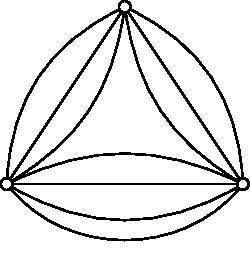
\includegraphics{image/introduction/Shannon-multigraphs_Sh7}
}
\caption{The family of Shannon multigraphs $\Sh(n)$ for $n = 2,\dots,7$.}
\label{fig:introduction:Shannon_multigraphs}
\end{figure}

\paragraph{Notational convention}
{\it
Unless stated otherwise, all graphs are simple graphs in the remainder
of this book.
}

\begin{definition}
For any vertex $v$ in a graph $G = (V, E)$, the
cardinality\index{cardinality} of $\adj(v)$ (as
in~\ref{eqn:introduction:directed_adjacency}) is called the
\emph{degree}\index{degree} of $v$ and written as
$\deg(v) = |\adj(v)|$\index{$\deg$}. The degree of $v$ counts the
number of vertices in $G$ that are adjacent to $v$. If $\deg(v) = 0$,
then $v$ is not incident to any edge and we say that $v$ is an
\emph{isolated}\index{vertex!isolated} vertex. If $G$ has no loops
and $\deg(v) = 1$, then $v$ is called a
\emph{pendant}\index{pendant}.
\end{definition}

Some examples would put the above definition in concrete
terms. Consider again the graph in
Figure~\ref{fig:introduction:self_loop}. Note that no vertices are
isolated. Even though vertex $a$ is not incident to any vertex other
than $a$ itself, note that $\deg(a) = 2$ and so by definition $a$ is
not isolated. Furthermore, each of $b$ and $c$ is a pendant. For the
house graph in Figure~\ref{fig:introduction:house_graph}, we have
$\deg(b) = 3$. For the graph in
Figure~\ref{fig:introduction:triangle_digraph}, we have
$\deg(b) = 2$. If $V \neq \emptyset$ and $E = \emptyset$, then
$G$ is a graph consisting entirely of isolated vertices. From
Example~\ref{eg:introduction:house_graph} we know that the vertices
$a, c, d$ in Figure~\ref{fig:introduction:house_graph} have the
smallest degree in the graph of that figure, while $b, e$ have the
largest degree.

The minimum\index{degree!minimum} degree\index{vertex!degree} among
all vertices in $G$ is denoted $\delta(G)$\index{$\delta(G)$}, whereas
the maximum\index{degree!maximum} degree is written as
$\Delta(G)$\index{$\Delta(G)$}. Thus, if $G$ denotes the graph in
Figure~\ref{fig:introduction:house_graph} then we have $\delta(G) = 2$
and $\Delta(G) = 3$. In the following Sage session, we construct the
digraph in Figure~\ref{fig:introduction:triangle_digraph} and compute
its maximum and minimum number of degrees.
\index{K\"onigsberg!seven bridges puzzle}
%%
\begin{lstlisting}
sage: G = DiGraph({"a":"b", "b":"c", "c":"a"})
sage: G
Digraph on 3 vertices
sage: G.degree("a")
2
sage: G.degree("b")
2
sage: G.degree("c")
2
\end{lstlisting}
%%
So for the graph $G$ in
Figure~\ref{fig:introduction:simple_graph_digraph_multidigraph}, we have
$\delta(G) = \Delta(G) = 2$.

The graph $G$ in
Figure~\ref{fig:introduction:simple_graph_digraph_multidigraph}
has the special property that its minimum degree is the same as its
maximum degree, i.e. $\delta(G) = \Delta(G)$. Graphs with this
property are referred to as
\emph{regular}\index{regular graph}. An
$r$-\emph{regular}\index{regular graph!$r$-regular}
graph is a regular graph each of whose vertices has degree $r$. For
instance, $G$ is a $2$-regular graph. The following result, due to
Euler, counts the total number of degrees in any graph.

\begin{theorem}
\label{thm:introduction:degree_sum}
\label{thm:introduction:hand_shaking}
\index{Euler!Leonhard}
\index{handshaking lemma}
\textbf{Euler 1736.}
If $G = (V, E)$ is a graph, then $\sum_{v \in V} \deg(v) = 2 |E|$.
\end{theorem}

\begin{proof}
Each edge $e = v_1 v_2 \in E$ is incident with two vertices, so $e$ is
counted twice towards the total sum of degrees. The first time, we
count $e$ towards the degree of vertex $v_1$ and the second time we
count $e$ towards the degree of $v_2$.
\end{proof}

Theorem~\ref{thm:introduction:hand_shaking} is sometimes called the
``handshaking lemma,'' due to its interpretation as in the following
story. Suppose you go into a room. Suppose there are $n$ people in the
room (including yourself) and some people shake hands with others and
some do not. Create the graph with $n$ vertices, where each vertex is
associated with a different person. Draw an edge between two people if
they shook hands. The degree of a vertex is the number of times that
person has shaken hands (we assume that there are no multiple edges,
i.e. that no two people shake hands twice). The theorem above simply
says that the total number of handshakes is even. This is ``obvious''
when you look at it this way since each handshake is counted twice
($A$ shaking $B$'s hand is counted, and $B$ shaking $A$'s hand is
counted as well, since the sum in the theorem is over all
vertices). To interpret Theorem~\ref{thm:introduction:hand_shaking} in
a slightly different way within the context of the same room of
people, there is an even number of people who shook hands with an odd
number of other people. This consequence of
Theorem~\ref{thm:introduction:hand_shaking} is recorded in the
following corollary.

\begin{corollary}
\label{cor:introduction:even_num_vertices_odd_degree}
A graph $G = (V, E)$ contains an even number of vertices with odd
degrees.
\end{corollary}

\begin{proof}
Partition $V$ into two disjoint subsets: $V_e$ is the subset of $V$
that contains only vertices with even degrees; and $V_o$ is the subset
of $V$ with only vertices of odd degrees. That is, $V = V_e \cup V_o$
and $V_e \cap V_o = \emptyset$. From
Theorem~\ref{thm:introduction:hand_shaking}, we have
\[
\sum_{v \in V} \deg(v)
=
\sum_{v \in V_e} \deg(v) + \sum_{v \in V_o} \deg(v)
=
2 |E|
\]
which can be re-arranged as
\[
\sum_{v \in V_o} \deg(v)
=
\sum_{v \in V} \deg(v) - \sum_{v \in V_e} \deg(v).
\]
As $\sum_{v \in V} \deg(v)$ and $\sum_{v \in V_e} \deg(v)$ are both
even, their difference is also even.
\end{proof}

As $E \subseteq V^{(2)}$, then $E$ can be the empty set, in which
case the total degree of $G = (V, E)$ is zero. Where $E \neq
\emptyset$, then the total degree of $G$ is greater than zero. By
Theorem~\ref{thm:introduction:degree_sum}, the total degree of $G$ is
nonnegative and even. This result is an immediate consequence of
Theorem~\ref{thm:introduction:degree_sum} and is captured in the
following corollary.

\begin{corollary}
\label{cor:introduction:degree_sum_even}
If $G$ is a graph, then the sum of its degrees is nonnegative
and even.
\end{corollary}

If $G = (V, E)$ is an $r$-regular graph with $n$ vertices and $m$
edges, it is clear by definition of $r$-regular graphs that the total
degree of $G$ is $rn$. By Theorem~\ref{thm:introduction:degree_sum} we
have $2m = rn$ and therefore $m = rn / 2$. This result is captured in
the following corollary.

\begin{corollary}
If $G = (V, E)$ is an $r$-regular graph having $n$ vertices and $m$
edges, then $m = rn / 2$.
\end{corollary}


%%%%%%%%%%%%%%%%%%%%%%%%%%%%%%%%%%%%%%%%%%%%%%%%%%%%%%%%%%%%%%%%%%%%%%%%%%%

\section{Subgraphs and other graph types}
\label{sec:introduction:subgraphs_graph_types}

We now consider several common types of graphs. Along the way, we also
present basic properties of graphs that could be used to distinguish
different types of graphs.

Let $G$ be a multigraph as in
Definition~\ref{def:introduction:graph-version3}, with vertex set
$V(G)$ and edge set $E(G)$. Consider a graph $H$ such that
$V(H) \subseteq V(G)$ and $E(H) \subseteq E(G)$. Furthermore, if
$e \in E(H)$ and $i(e) = \{u,v\}$, then $u,v \in V(H)$. Under these
conditions, $H$ is called a \emph{subgraph}\index{subgraph} of $G$.


%%%%%%%%%%%%%%%%%%%%%%%%%%%%%%%%%%%%%%%%%%%%%%%%%%%%%%%%%%%%%%%%%%%%%%%%%%%

%\newpage
\subsection{Walks, trails, and paths}
\label{subsec:introduction:walks_trails_paths}

\begin{quote}
\footnotesize
I like long walks, especially when they are taken by people who annoy
me. \\
\noindent
--- Noel Coward\index{Coward, Noel}
\end{quote}

\noindent
If $u$ and $v$ are two vertices in a graph $G$, a $u$-$v$
\emph{walk}\index{walk} is an alternating sequence of vertices and
edges starting with $u$ and ending at $v$. Consecutive vertices and
edges are incident. Formally, a \emph{walk}\index{walk} $W$ of length
$n \geq 0$ can be defined as
\[
W: v_0, e_1, v_1, e_2, v_2, \dots, v_{n-1}, e_n, v_n
\]
where each edge $e_i = v_{i-1} v_i$ and the length\index{walk!length}
$n$ refers to the number of~(not necessarily distinct) edges in the
walk. The vertex $v_0$ is the starting vertex of the walk and $v_n$ is
the end vertex, so we refer to $W$ as a $v_0$-$v_n$ walk. The
\emph{trivial walk}\index{walk!trivial} is the walk of length $n = 0$
in which the start and end vertices are one and the same vertex. If
the graph has no multiple edges then, for brevity, we omit the edges
in a walk and usually write the walk as the following sequence of
vertices:
\[
W: v_0, v_1, v_2, \dots, v_{n-1}, v_n.
\]
For the graph in Figure~\ref{fig:introduction:types_of_walks}, an
example of a walk is an $a$-$e$ walk: $a, b, c, b, e$. In other words,
we start at vertex $a$ and travel to vertex $b$. From $b$, we go to
$c$ and then back to $b$ again. Then we end our journey at $e$. Notice
that consecutive vertices in a walk are adjacent to each other. One
can think of vertices as destinations and edges as footpaths, say. We
are allowed to have repeated vertices and edges in a walk. The number
of edges in a walk is called its \emph{length}\index{walk!length}. For
instance, the walk $a, b, c, b, e$ has length $4$.

\begin{figure}[!htbp]
\centering
\includegraphics{image/introduction/types-of-walks}
\caption{Walking along a graph.}
\label{fig:introduction:types_of_walks}
\end{figure}

A \emph{trail}\index{trail} is a walk with no repeating edges. For
example, the $a$-$b$ walk $a, b, c, d, f, g, b$ in
Figure~\ref{fig:introduction:types_of_walks} is a trail. It does not
contain any repeated edges, but it contains one repeated vertex,
i.e. $b$. Nothing in the definition of a trail restricts a trail from
having repeated vertices. A walk with no repeating vertices, except
possibly the first and last, is called a \emph{path}\index{path}.
Without any repeating vertices, a path cannot have repeating edges,
hence a path is also a trail.

\begin{proposition}
\label{prop:introduction:any_path_has_length_at_most_n_minus_1}
Let $G = (V, E)$ be a simple (di)graph of order $n = |V|$. Any path in $G$
has length at most $n - 1$.
\end{proposition}

\begin{proof}
Let $V = \{v_1, v_2, \dots, v_n\}$ be the vertex set of $G$. Without
loss of generality, we can assume that each pair of vertices in
the digraph $G$ is connected by an edge, giving a total of $n^2$
possible edges for $E = V \times V$. We can remove self-loops from
$E$, which now leaves us with an edge set $E_1$ that consists of
$n^2 - n$ edges. Start our path from any vertex, say, $v_1$. To
construct a path of length $1$, choose an edge $v_1 v_{j_1} \in E_1$
such that $v_{j_1} \notin \{v_1\}$. Remove from $E_1$ all $v_1 v_k$
such that $v_{j_1} \neq v_k$. This results in a reduced edge set $E_2$
of $n^2 - n - (n - 2)$ elements and we now have the path
$P_1: v_1, v_{j_1}$ of length $1$. Repeat the same process for
$v_{j_1} v_{j_2} \in E_2$ to obtain a reduced edge set $E_3$ of
$n^2 - n - 2(n - 2)$ elements and a path $P_2: v_1, v_{j_1}, v_{j_2}$
of length $2$. In general, let
$P_r: v_1, v_{j_1}, v_{j_2}, \dots, v_{j_r}$ be a path of length
$r < n$ and let $E_{r+1}$ be our reduced edge set of
$n^2 - n - r(n - 2)$ elements. Repeat the above process until we have
constructed a path
$P_{n-1}: v_1, v_{j_1}, v_{j_2}, \dots, v_{j_{n-1}}$ of length $n - 1$
with reduced edge set $E_n$ of $n^2 - n - (n - 1)(n - 2)$
elements. Adding another vertex to $P_{n-1}$ means going back to a
vertex that was previously visited, because $P_{n-1}$ already contains
all vertices of $V$.
\end{proof}

A walk\index{walk} of length $n \geq 3$ whose start and end vertices
are the same is called a \emph{closed walk}\index{walk!closed}.
A trail\index{trail} of length $n \geq 3$ whose start and end vertices
are the same is called a \emph{closed trail}\index{trail!closed}.
A path\index{path} of length $n \geq 3$ whose start and end vertices
are the same is called a \emph{closed path}\index{path!closed}
or a \emph{cycle}\index{cycle}~(with apologies for slightly abusing
terminology).\footnote{
  A cycle in a graph is sometimes also called a
  ``circuit''\index{circuit}. Since that terminology unfortunately
  conflicts with the closely related notion of a circuit of a matroid,
  we do not use it here.
}
For example, the walk $a, b, c, e, a$ in
Figure~\ref{fig:introduction:types_of_walks} is a closed path. A path
whose length is odd is called \emph{odd}\index{path!odd}, otherwise it
is referred to as \emph{even}\index{path!even}. Thus the walk
$a, b, e, a$ in Figure~\ref{fig:introduction:types_of_walks} is a
cycle. It is easy to see that if you remove any edge from a cycle,
then the resulting walk contains no closed walks. An
\emph{Euler subgraph}\index{Euler!subgraph} of a graph $G$ is either a
cycle or an edge-disjoint union of cycles in $G$. An example of a
closed walk which is not a cycle is given in
Figure~\ref{fig:introduction:butterfly_graph}.

\begin{figure}[!htbp]
\centering
\index{bowtie graph}
\index{butterfly graph}
\includegraphics{image/introduction/butterfly-graph}
\caption{Butterfly graph with $5$ vertices.}
\label{fig:introduction:butterfly_graph}
\end{figure}

The length of the shortest cycle in a graph is called the
\emph{girth}\index{girth} of the graph. By convention, an acyclic
graph is said to have infinite girth.

\begin{example}
\label{eg:introduction:walks_paths_trails}
Consider the graph in Figure~\ref{fig:introduction:types_of_walks}.
%%
\begin{enumerate}
\item Find two distinct walks that are not trails and determine their
  lengths.

\item Find two distinct trails that are not paths and determine their
  lengths.

\item Find two distinct paths and determine their lengths.

\item Find a closed trail that is not a cycle.

\item Find a closed walk $C$ which has an edge $e$ such that $C - e$
  contains a cycle.
\end{enumerate}
\end{example}

\begin{proof}[Solution]
(1)~Here are two distinct walks that are not trails:
$w_1: g, b, e, a, b, e$ and $w_2: f, d, c, e, f, d$. The length of
walk $w_1$ is 5 and the length of walk $w_2$ is also 5.

(2)~Here are two distinct trails that are not paths:
$t_1: a,b,c,e,b$ and $t_2: b,e,f,d,c,e$. The length of trail $t_1$ is
4 and the length of trail $t_2$ is 5.

(3)~Here are two distinct paths: $p_1: a, b, c, d, f, e$ and
$p_2: g, b, a, e, f, d$. The length of path $p_1$ is 5 and the length
of path $p_2$ is also 5.

(4)~Here is a closed trail that is not a cycle: $d, c, e, b, a, e, f, d$.

(5)~Left to the reader.
\end{proof}

\begin{theorem}
\label{thm:introduction:every_walk_has_a_path}
Every $u$-$v$ walk in a graph contains a $u$-$v$ path.
\end{theorem}

\begin{proof}
A walk of length $n = 0$ is the trivial path. So assume that $W$ is a
$u$-$v$ walk of length $n > 0$ in a graph $G$:
\[
W: u = v_0, v_1, \dots, v_n = v.
\]
It is possible that a vertex in $W$ is assigned two different
labels. If $W$ has no repeated vertices, then $W$ is already a
path. Otherwise $W$ has at least one repeated vertex. Let
$0 \leq i,j \leq n$ be two distinct integers with $i < j$ such that
$v_i = v_j$. Deleting the vertices $v_i, v_{i+1}, \dots, v_{j-1}$ from
$W$ results in a $u$-$v$ walk $W_1$ whose length is less than $n$. If
$W_1$ is a path, then we are done. Otherwise we repeat the above
process to obtain a $u$-$v$ walk shorter than $W_1$. As $W$ is a
finite sequence, we only need to apply the above process a finite
number of times to arrive at a $u$-$v$ path.
\end{proof}

A graph is said to be
\emph{connected}\index{connected graph}\index{graph!connected} if for
every pair of distinct vertices $u, v$ there is a $u$-$v$ path joining
them. A graph that is not connected is referred to as
\emph{disconnected}\index{disconnected graph}\index{graph!disconnected}.
The empty graph is disconnected and so is any nonempty graph with an
isolated vertex. However, the graph in
Figure~\ref{fig:introduction:simple_graph_digraph_multidigraph} is
connected. A \emph{geodesic path}\index{path!geodesic} or
\emph{shortest path}\index{shortest path} between two distinct
vertices $u,v$ of a graph is a $u$-$v$ path of minimum length. A
nonempty graph may have several shortest paths between some distinct
pair of vertices. For the graph in
Figure~\ref{fig:introduction:types_of_walks}, both $a,b,c$ and $a,e,c$
are geodesic paths between $a$ and $c$. Let $H$ be a connected
subgraph of a graph $G$ such that $H$ is not a proper subgraph of any
connected subgraph of $G$. Then $H$ is said to be a
\emph{component}\index{component} of $G$. We also say that $H$ is a
maximal connected subgraph of $G$. Any connected graph is its own
component. The number of connected components of a graph $G$ will be
denoted $\omega(G)$\index{$\omega$}.

The following is an immediate consequence of
Corollary~\ref{cor:introduction:even_num_vertices_odd_degree}.

\begin{proposition}
Suppose that exactly two vertices of a graph have odd degree. Then
those two vertices are connected by a path.
\end{proposition}

\begin{proof}
Let $G$ be a graph all of whose vertices are of even degree, except
for $u$ and $v$. Let $C$ be a component of $G$ containing $u$. By
Corollary~\ref{cor:introduction:even_num_vertices_odd_degree}, $C$
also contains $v$, the only remaining vertex of odd degree. As $u$ and
$v$ belong to the same component, they are connected by a path.
\end{proof}

\begin{example}
Determine whether or not the graph in
Figure~\ref{fig:introduction:types_of_walks} is connected. Find a
shortest path from $g$ to $d$.
\end{example}

\begin{proof}[Solution]
In the following Sage session, we first construct the graph in
Figure~\ref{fig:introduction:types_of_walks} and use the method
\verb!is_connected()! to determine whether or not the graph is
connected. Finally, we use the method \verb!shortest_path()! to find
a geodesic path between $g$ and $d$.
%%
\begin{lstlisting}
sage: g = Graph({"a":["b","e"], "b":["a","g","e","c"], \
...   "c":["b","e","d"], "d":["c","f"], "e":["f","a","b","c"], \
...   "f":["g","d","e"], "g":["b","f"]})
sage: g.is_connected()
True
sage: g.shortest_path("g", "d")
['g', 'f', 'd']
\end{lstlisting}
%%
This shows that $g, f, d$ is a shortest path from $g$ to $d$. In fact,
any other $g$-$d$ path has length greater than $2$, so we can say that
$g, f, d$ is the shortest path between $g$ and $d$.
\end{proof}

\begin{remark}
\rm
We will explain Dijkstra's\index{Dijkstra!algorithm} algorithm in
Chapter~\ref{chap:graph_algorithms}, which gives one of the best
algorithms for finding shortest paths between two vertices in a
connected graph. What is very remarkable is that, at the present state
of knowledge, finding the shortest path from a vertex $v$ to a
\emph{particular} (but arbitrarily given) vertex $w$ appears to be as
hard as finding the shortest path from a vertex $v$ to \emph{all}
other vertices in the graph!
\end{remark}

Trees are a special type of graphs that are used in modelling
structures that have some form of
hierarchy\index{hierarchical structure}. For example, the hierarchy
within an organization can be drawn as a tree structure, similar to
the family tree in
Figure~\ref{fig:introduction:family_tree}\index{family tree}.
Formally, a \emph{tree}\index{tree} is an undirected graph that is
connected and has no cycles. If one vertex of a tree is specially
designated as the \emph{root vertex}\index{vertex!root}, then the tree
is called a  \emph{rooted tree}\index{tree!rooted}.
Chapter~\ref{chap:trees_forests} covers trees in more details.

\begin{figure}[!htbp]
\centering
\index{family tree}
\includegraphics{image/introduction/family-tree}
\caption{A family tree.}
\label{fig:introduction:family_tree}
\end{figure}


%%%%%%%%%%%%%%%%%%%%%%%%%%%%%%%%%%%%%%%%%%%%%%%%%%%%%%%%%%%%%%%%%%%%%%%%%%%

\subsection{Subgraphs, complete and bipartite graphs}
\index{subgraph}

Let $G$ be a graph with vertex set $V(G)$ and edge set $E(G)$. Suppose
we have a graph $H$ such that $V(H) \subseteq V(G)$ and
$E(H) \subseteq E(G)$. Furthermore, suppose the incidence function $i$
of $G$, when restricted to $E(H)$, has image in $V(H)^{(2)}$. Then $H$
is a \emph{subgraph}\index{subgraph} of $G$. In this situation, $G$ is
referred to as a \emph{supergraph}\index{supergraph} of $H$.

Starting from $G$, one can obtain its subgraph $H$ by deleting edges
and/or vertices from $G$. Note that when a vertex $v$ is removed from
$G$, then all edges incident with $v$ are also removed. If
$V(H) = V(G)$, then $H$ is called a
\emph{spanning subgraph}\index{spanning subgraph} of $G$. In
Figure~\ref{fig:introduction:star_subgraph}, let $G$ be the left-hand
side graph and let $H$ be the right-hand side graph. Then it is clear
that $H$ is a spanning subgraph of $G$. To obtain a spanning subgraph
from a given graph, we delete edges from the given graph.

\begin{figure}[!htbp]
\centering
\subfigure[]{
  \includegraphics{image/introduction/star-subgraph_pentagon-star}
}
\qquad
\subfigure[]{
  \includegraphics{image/introduction/star-subgraph_star}
}
\caption{A graph and one of its subgraphs.}
\label{fig:introduction:star_subgraph}
\end{figure}

We now consider several standard classes of graphs. The
\emph{complete graph}\index{complete graph} $K_n$\index{$K_n$} on $n$
vertices is a graph such that any two distinct vertices are
adjacent. As $|V(K_n)| = n$, then $|E(K_n)|$ is equivalent to the
total number of 2-combinations from a set of $n$ objects:
%%
\begin{equation}
\label{eqn:introduction:size_of_K_n}
|E(K_n)|
=
\binom{n}{2}
=
\frac{n(n-1)}{2}.
\end{equation}
%%
Thus for any simple graph $G$ with $n$ vertices, its total number of
edges $|E(G)|$ is bounded above by
%%
\begin{equation}
\label{eqn:introduction:upper_bound_total_edges_simple_graph}
|E(G)|
\leq
\frac{n(n - 1)}{2}.
\end{equation}
%%
Figure~\ref{fig:introduction:five_complete_graphs} shows complete
graphs each of whose total number of vertices is bounded by
$1 \leq n \leq 5$. The complete graph $K_1$ has one vertex with
no edges. It is also called the
\emph{trivial graph}\index{trivial graph}.

\begin{figure}[!htbp]
\centering
\index{complete graph}
\subfigure[$K_5$]{
  \includegraphics{image/introduction/five-complete-graphs_pentagon}
}
\quad
\subfigure[$K_4$]{
\label{fig:five_complete_graphs:complete_graph_on_four_vertices}
  \includegraphics{image/introduction/five-complete-graphs_rectangle}
}
\quad
\subfigure[$K_3$]{
  \includegraphics{image/introduction/five-complete-graphs_triangle}
}
\quad
\subfigure[$K_2$]{
  \includegraphics{image/introduction/five-complete-graphs_line}
}
\quad
\subfigure[$K_1$]{
  \includegraphics{image/introduction/five-complete-graphs_point}
}
\caption{Complete graphs $K_n$ for $1 \leq n \leq 5$.}
\label{fig:introduction:five_complete_graphs}
\end{figure}

The following result is an application of
inequality~\eqref{eqn:introduction:upper_bound_total_edges_simple_graph}.

\begin{theorem}
Let $G$ be a simple graph with $n$ vertices and $k$ components. Then
$G$ has at most $\frac{1}{2} (n - k)(n - k + 1)$ edges.
\end{theorem}

\begin{proof}
If $n_i$ is the number of vertices in component $i$, then $n_i > 0$
and it can be shown~(see the proof of Lemma~2.1
in~\cite[pp.21--22]{Foulds1992}) that
%%
\begin{equation}
\label{eqn:introduction:inequality_set_positive_integers}
\sum n_i^2
\leq
\left(\sum n_i\right)^2 - (k - 1) \left(2 \sum n_i - k\right).
\end{equation}
%%
(This result holds true for any nonempty but finite set of positive
integers.) Note that $\sum n_i = n$ and
by~\eqref{eqn:introduction:upper_bound_total_edges_simple_graph} each
component $i$ has at most $\frac{1}{2} n_i (n_i - 1)$
edges. Apply~\eqref{eqn:introduction:inequality_set_positive_integers}
to get
%%
\begin{align*}
\sum \frac{n_i (n_i - 1)}{2}
&=
\frac{1}{2} \sum n_i^2 - \frac{1}{2} \sum n_i \\[4pt]
&\leq
\frac{1}{2} (n^2 - 2nk + k^2 + 2n - k) - \frac{1}{2} n \\[4pt]
&=
\frac{(n - k) (n - k + 1)}{2}
\end{align*}
%%
as required.
\end{proof}

The \emph{cycle graph}\index{cycle graph} on $n \geq 3$ vertices,
denoted $C_n$\index{$C_n$}, is the connected $2$-regular graph on $n$
vertices. Each vertex in $C_n$ has degree exactly $2$ and $C_n$ is
connected. Figure~\ref{fig:introduction:four_cycle_graphs} shows
cycles graphs $C_n$ where $3 \leq n \leq 6$. The
\emph{path graph}\index{path graph} on $n \geq 1$ vertices is denoted
$P_n$\index{$P_n$}. For $n = 1, 2$ we have $P_1 = K_1$ and
$P_2 = K_2$. Where $n \geq 3$, then $P_n$ is a spanning subgraph of
$C_n$ obtained by deleting one edge.

\begin{figure}[!htbp]
\centering
\index{cycle graph}
\subfigure[$C_6$]{
  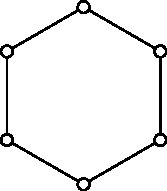
\includegraphics{image/introduction/four-cycle-graphs_hexagon}
}
\quad
\subfigure[$C_5$]{
  \includegraphics{image/introduction/four-cycle-graphs_pentagon}
}
\quad
\subfigure[$C_4$]{
  \includegraphics{image/introduction/four-cycle-graphs_square}
}
\quad
\subfigure[$C_3$]{
  \includegraphics{image/introduction/four-cycle-graphs_triangle}
}
\caption{Cycle graphs $C_n$ for $3 \leq n \leq 6$.}
\label{fig:introduction:four_cycle_graphs}
\end{figure}

A \emph{bipartite graph}\index{bipartite graph} $G$ is a graph with at
least two vertices such that $V(G)$ can be split into two disjoint
subsets $V_1$ and $V_2$, both nonempty. Every edge $uv \in E(G)$ is
such that $u \in V_1$ and $v \in V_2$, or $v \in V_1$ and $u \in V_2$.
See Kalman~\cite{Kalman1999} for an application of bipartite graphs to
the problem of allocating satellites to radio stations.

\begin{theorem}
A graph is bipartite if and only if it has no odd cycles.
\end{theorem}

\begin{proof}
Necessity~($\Longrightarrow$): Assume $G$ to be bipartite. Traversing
each edge involves going from one side of the bipartition to the
other. For a walk to be closed, it must have even length in order to
return to the side of the bipartition from which the walk
started. Thus, any cycle in $G$ must have even length.

Sufficiency~($\Longleftarrow$): Assume $G = (V, E)$ has order
$n \geq 2$ and no odd cycles. If $G$ is connected, choose any vertex
$u \in V$ and define a partition of $V$ thus:
%%
\begin{align*}
X &= \{x \in V \mid d(u,x) \text{ is even}\}, \\
Y &= \{y \in V \mid d(u,y) \text{ is odd}\}
\end{align*}
%%
where $d(u,v)$ denotes the distance (or length of the shortest path)
from $u$ to $v$. If $(X, Y)$ is a bipartition of $G$, then we are
done. Otherwise, $(X, Y)$ is not a bipartition of $G$. Then one of $X$
and $Y$ has two vertices $v,w$ joined by an edge $e$. Let $P_1$ be a
shortest $u$-$v$ path and $P_2$ be a shortest $u$-$w$ path. By
definition of $X$ and $Y$, both $P_1$ and $P_2$ have even lengths or
both have odd lengths. From $u$, let $x$ be the last vertex common to
both $P_1$ and $P_2$. The subpath $u$-$x$ of $P_1$ and $u$-$x$ of
$P_2$ have equal length. That is, the subpath $x$-$v$ of $P_1$ and
$x$-$w$ of $P_2$ both have even or odd lengths. Construct a cycle $C$
from the paths $x$-$v$ and $x$-$w$, and the edge $e$ joining $v$ and
$w$. Since $x$-$v$ and $x$-$w$ both have even or odd lengths, the
cycle $C$ has odd length, contradicting our hypothesis that $G$ has no
odd cycles. Hence, $(X,Y)$ is a bipartition of $G$.

Finally, if $G$ is disconnected, each of its components has no odd
cycles. Repeat the above argument for each component to conclude that
$G$ is bipartite.
\end{proof}

The \emph{complete bipartite}\index{bipartite graph!complete} graph
$K_{m,n}$\index{$K_{m,n}$} is the bipartite graph whose vertex set is
partitioned into two nonempty disjoint sets $V_1$ and $V_2$ with
$|V_1| = m$ and $|V_2| = n$. Any vertex in $V_1$ is adjacent to each
vertex in $V_2$, and any two distinct vertices in $V_i$ are not
adjacent to each other. If $m = n$, then $K_{n,n}$ is
$n$-regular. Where $m = 1$ then $K_{1,n}$ is called the
\emph{star graph}\index{star graph}.
Figure~\ref{fig:introduction:bipartite_complete_bipartite_graphs}
shows a bipartite graph together with the complete bipartite graphs
$K_{4,3}$ and $K_{3,3}$, and the star graph $K_{1,4}$.

\begin{figure}[!htbp]
\centering
\index{bipartite graph!complete}
\index{bipartite graph}
\index{star graph}
\subfigure[bipartite]{
  \includegraphics{image/introduction/bipartite-complete-bipartite-graphs_bipartite}
}
\quad
\subfigure[$K_{4,3}$]{
  \includegraphics{image/introduction/bipartite-complete-bipartite-graphs_K43}
}
\quad
\subfigure[$K_{3,3}$]{
  \includegraphics{image/introduction/bipartite-complete-bipartite-graphs_K33}
}
\quad
\subfigure[$K_{1,4}$]{
  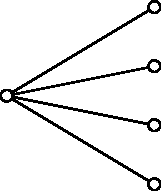
\includegraphics{image/introduction/bipartite-complete-bipartite-graphs_K14}
}
\caption{Bipartite, complete bipartite, and star graphs.}
\label{fig:introduction:bipartite_complete_bipartite_graphs}
\end{figure}

As an example of $K_{3,3}$, suppose that there are $3$ boys and $3$
girls dancing in a room. The boys and girls naturally partition the
set of all people in the room. Construct a graph having $6$ vertices,
each vertex corresponding to a person in the room, and draw an edge
form one vertex to another if the two people dance together. If each
girl dances three times, once with with each of the three boys, then
the resulting graph is $K_{3,3}$.


%%%%%%%%%%%%%%%%%%%%%%%%%%%%%%%%%%%%%%%%%%%%%%%%%%%%%%%%%%%%%%%%%%%%%%%%%%%

\section{Representing graphs as matrices}
\label{sec:introduction:matrix_representation}

\begin{quote}
\footnotesize
Neo: What is the Matrix? \\
Morpheus: Unfortunately, no one can be told what the Matrix is. You
have to see it for yourself. \\
\noindent
--- From the movie \emph{The Matrix}, 1999
\end{quote}

\noindent
An $m \times n$ matrix\index{matrix} $A$ can be represented as
\[
A
=
\begin{bmatrix}
a_{11} & a_{12} & \cdots & a_{1n} \\
a_{21} & a_{22} & \cdots & a_{2n} \\
\hdotsfor{4} \\
a_{m1} & a_{m2} & \cdots & a_{mn} \\
\end{bmatrix}.
\]
The positive integers $m$ and $n$ are the row and column dimensions of
$A$, respectively. The entry in row $i$ column $j$ is denoted
$a_{ij}$. Where the dimensions of $A$ are clear from context, $A$ is
also written as $A = [a_{ij}]$.

Representing a graph as a matrix is very inefficient in some cases and
not so in other cases. Imagine you walk into a large room full of
people and you consider the ``handshaking graph'' discussed in
connection with Theorem~\ref{thm:introduction:hand_shaking}. If not
many people shake hands in the room, it is a waste of time recording
all the handshakes and also all the ``non-handshakes.'' This is
basically what the adjacency matrix does. In this kind of
``sparse graph''\index{graph!sparse} situation, it would be much
easier to simply record the handshakes as a Python
dictionary.\footnote{
  A Python\index{Python} dictionary is basically an indexed set. See
  the reference manual at \url{http://www.python.org} for further
  details.
}
This section requires some concepts and techniques from linear
algebra, especially matrix theory. See introductory texts on linear
algebra and matrix theory~\cite{Beezer2009} for coverage of such
concepts and techniques.


%%%%%%%%%%%%%%%%%%%%%%%%%%%%%%%%%%%%%%%%%%%%%%%%%%%%%%%%%%%%%%%%%%%%%%%%%%%

\subsection{Adjacency matrix}

Let $G$ be an undirected graph with vertices
$V = \{ v_1, \dots, v_n \}$ and edge set $E$. The
\emph{adjacency matrix} of $G$ is the $n \times n$ matrix
$A = [a_{ij}]$ defined by
\[
a_{ij}
=
\begin{cases}
1, & \text{if $v_i v_j \in E$}, \\[4pt]
0, & \text{otherwise}.
\end{cases}
\]
As $G$ is an undirected graph, then $A$ is a symmetric matrix. That
is, $A$ is a square matrix such that $a_{ij} = a_{ji}$.

Now let $G$ be a directed graph with vertices
$V = \{ v_1, \dots, v_n \}$ and edge set $E$. The
$(0, -1, 1)$-\emph{adjacency matrix}\index{adjacency matrix} of $G$ is
the $n \times n$ matrix $A = [a_{ij}]$ defined by
\[
a_{ij}
=
\begin{cases}
1,  & \text{if $v_i v_j \in E$}, \\[4pt]
-1, & \text{if $v_j v_i \in E$}, \\[4pt]
0,  & \text{otherwise}.
\end{cases}
\]

\begin{figure}[!htbp]
\centering
\index{matrix!adjacency}
\subfigure[]{
  \includegraphics{image/introduction/adjacency-matrices_directed}
}
\qquad
\subfigure[]{
  \includegraphics{image/introduction/adjacency-matrices_undirected}
}
\caption{What are the adjacency matrices of these graphs?}
\label{fig:introduction:adjacency_matrices}
\end{figure}

\begin{example}
Compute the adjacency matrices of the graphs in
Figure~\ref{fig:introduction:adjacency_matrices}.
\end{example}

\begin{proof}[Solution]
Define the graphs in Figure~\ref{fig:introduction:adjacency_matrices}
using \verb!DiGraph! and \verb!Graph!. Then call the method
\verb!adjacency_matrix()!.
%%
\begin{lstlisting}
sage: G1 = DiGraph({1:[2], 2:[1], 3:[2,6], 4:[1,5], 5:[6], 6:[5]})
sage: G2 = Graph({"a":["b","c"], "b":["a","d"], "c":["a","e"], \
...   "d":["b","f"], "e":["c","f"], "f":["d","e"]})
sage: m1 = G1.adjacency_matrix(); m1
[0 1 0 0 0 0]
[1 0 0 0 0 0]
[0 1 0 0 0 1]
[1 0 0 0 1 0]
[0 0 0 0 0 1]
[0 0 0 0 1 0]
sage: m2 = G2.adjacency_matrix(); m2
[0 1 1 0 0 0]
[1 0 0 1 0 0]
[1 0 0 0 1 0]
[0 1 0 0 0 1]
[0 0 1 0 0 1]
[0 0 0 1 1 0]
sage: m1.is_symmetric()
False
sage: m2.is_symmetric()
True
\end{lstlisting}
%%
In general, the adjacency matrix of a digraph is not symmetric, while
that of an undirected graph is symmetric.
\end{proof}

%% \begin{theorem}
%% Let $G$ be a graph of order $n$ and $\mathbf{A}$ the adjacency matrix
%% of $G$. For each positive integer $k$, the $i$-$j$ entry of
%% $\mathbf{A}^k$ counts the number of $v_i$-$v_j$ walks of length $k$.
%% \end{theorem}

More generally, if $G$ is an undirected multigraph with edge
$e_{ij} = v_i v_j$ having multiplicity $w_{ij}$, or a weighted
graph with edge $e_{ij} = v_i v_j$ having weight $w_{ij}$, then we
can define the (weighted) \emph{adjacency matrix} $A = [a_{ij}]$ by
\[
a_{ij}
=
\begin{cases}
w_{ij}, & \text{if $v_i v_j \in E$}, \\[4pt]
0,      & \text{otherwise}.
\end{cases}
\]
For example, Sage allows you to easily compute a weighted adjacency
matrix.
%%
\begin{lstlisting}
sage: G = Graph(sparse=True, weighted=True)
sage: G.add_edges([(0,1,1), (1,2,2), (0,2,3), (0,3,4)])
sage: M = G.weighted_adjacency_matrix(); M
[0 1 3 4]
[1 0 2 0]
[3 2 0 0]
[4 0 0 0]
\end{lstlisting}


%%%%%%%%%%%%%%%%%%%%%%%%%%%%%%%%%%%%%%%%%%%%%%%%%%%%%%%%%%%%%%%%%%%%%%%%%%%

\subsubsection{Bipartite case}

Suppose $G = (V, E)$ is an undirected bipartite graph and
$V = V_1 \cup V_2$ is the partition of the vertices into $n_1$
vertices in $V_1$ and $n_2$ vertices in $V_2$, so $|V| = n_1 + n_2$.
Then the adjacency matrix $A$ of $G$ can be realized as a block
diagonal matrix
$A
=
\begin{bmatrix}
A_1 & 0 \\
0 & A_2
\end{bmatrix}$,
where $A_1$ is an $n_1 \times n_2$ matrix and $A_2$ is an
$n_2 \times n_1$ matrix. Since $G$ is undirected, $A_2 = A_1^T$.
The matrix is called a
\emph{reduced adjacency matrix}\index{adjacency matrix!reduced} or a
\emph{bi-adjacency matrix}\index{matrix!bi-adjacency}~(the literature
also uses the terms ``transfer matrix'' or the ambiguous term
``adjacency matrix'').


%%%%%%%%%%%%%%%%%%%%%%%%%%%%%%%%%%%%%%%%%%%%%%%%%%%%%%%%%%%%%%%%%%%%%%%%%%%

\subsubsection{Tanner graphs}

If $H$ is an $m \times n$ $(0,1)$-matrix, then the
\emph{Tanner graph}\index{Tanner graph} of $H$ is the bipartite graph
$G = (V,E)$ whose set of vertices $V = V_1 \cup V_2$ is partitioned
into two sets: $V_1$ corresponding to the $m$ rows of $H$ and $V_2$
corresponding to the $n$ columns of $H$. For any $i,j$ with
$1 \leq i \leq m$ and $1 \leq j \leq n$, there is an edge $ij \in E$
if and only if the $(i,j)$-th entry of $H$ is $1$. This matrix $H$ is
sometimes called the reduced adjacency matrix or the
\emph{check matrix}\index{check matrix} of the
Tanner\index{Tanner graph} graph. Tanner graphs are used in the theory
of error-correcting\index{code!error-correcting} codes. For example,
Sage allows you to easily compute such a bipartite graph from its
matrix.
%%
\begin{lstlisting}
sage: H = Matrix([(1,1,1,0,0), (0,0,1,0,1), (1,0,0,1,1)])
sage: B = BipartiteGraph(H)
sage: B.reduced_adjacency_matrix()
[1 1 1 0 0]
[0 0 1 0 1]
[1 0 0 1 1]
sage: B.plot(graph_border=True)
\end{lstlisting}
%%
The corresponding graph is similar to that in
Figure~\ref{fig:introduction:tanner_graph}.

\begin{figure}[!htbp]
\centering
\index{Tanner graph}
\includegraphics{image/introduction/tanner-graph}
\caption{A Tanner graph.}
\label{fig:introduction:tanner_graph}
\end{figure}

\begin{theorem}
Let $A$ be the adjacency matrix of a graph $G$ with vertex set
$V = \{v_1, v_2, \dots, v_p\}$. For each positive integer $n$, the
$ij$-th entry of $A^n$ counts the number of $v_i$-$v_j$ walks of
length $n$ in $G$.
\end{theorem}

\begin{proof}
We shall prove by induction on $n$. For the base case $n = 1$, the
$ij$-th entry of $A^1$ counts the number of walks of length 1 from
$v_i$ to $v_j$. This is obvious because $A^1$ is merely the adjacency
matrix $A$.

Suppose for induction that for some positive integer $k \geq 1$, the
$ij$-th entry of $A^k$ counts the number of walks of length $k$ from
$v_i$ to $v_j$. We need to show that the $ij$-th entry of $A^{k+1}$
counts the number of $v_i$-$v_j$ walks of length $k + 1$. Let
$A = [a_{ij}]$, $A^k = [b_{ij}]$, and $A^{k+1} = [c_{ij}]$. Since
$A^{k+1} = A A^k$, then
\[
c_{ij}
=
\sum_{r=1}^p a_{ir} b_{rj}
\]
for $i,j = 1, 2, \dots, p$. Note that $a_{ir}$ is the number of edges
from $v_i$ to $v_r$, and $b_{rj}$ is the number of $v_r$-$v_j$ walks
of length $k$. Any edge from $v_i$ to $v_r$ can be joined with any
$v_r$-$v_j$ walk to create a walk $v_i, v_r, \dots, v_j$ of length
$k + 1$. Then for each $r = 1, 2, \dots, p$, the value $a_{ir} b_{rj}$
counts the number of $v_i$-$v_j$ walks of length $k + 1$ with $v_r$
being the second vertex in the walk. Thus $c_{ij}$ counts the total
number of $v_i$-$v_j$ walks of length $k + 1$.
\end{proof}


%%%%%%%%%%%%%%%%%%%%%%%%%%%%%%%%%%%%%%%%%%%%%%%%%%%%%%%%%%%%%%%%%%%%%%%%%%%

\subsection{Incidence matrix}

The relationship between edges and vertices provides a very strong
constraint on the data structure, much like the relationship between
points and blocks in a combinatorial design or points and lines in a
finite plane geometry. This incidence structure gives rise to another
way to describe a graph using a matrix.

Let $G$ be a digraph with edge set $E = \{ e_1, \dots, e_m \}$ and
vertex set $V = \{ v_1, \dots, v_n \}$. The
\emph{incidence matrix}\index{incidence!matrix} of $G$ is the
$n \times m$ matrix $B = [b_{ij}]$ defined by
%%
\begin{equation}
\label{eqn:introduction:incidence_matrix_digraph}
b_{ij}
=
\begin{cases}
-1, & \text{if $v_i$ is the tail of $e_j$}, \\[4pt]
1,  & \text{if $v_i$ is the head of $e_j$}, \\[4pt]
2,  & \text{if $e_j$ is a self-loop at $v_i$}, \\[4pt]
0,  & \text{otherwise}.
\end{cases}
\end{equation}
%%
Each column of $B$ corresponds to an edge and each row corresponds to
a vertex. The definition of incidence matrix of a digraph as contained
in expression~\eqref{eqn:introduction:incidence_matrix_digraph} is
applicable to digraphs with self-loops as well as multidigraphs.

For the undirected case, let $G$ be an undirected graph with edge set
$E = \{ e_1, \dots, e_m \}$ and vertex set
$V = \{ v_1, \dots, v_n \}$. The
\emph{unoriented incidence matrix}\index{incidence matrix!unoriented}
of $G$ is the $n \times m$ matrix $B = [b_{ij}]$ defined by
\[
b_{ij}
=
\begin{cases}
1, & \text{if $v_i$ is incident to $e_j$}, \\[4pt]
2, & \text{if $e_j$ is a self-loop at $v_i$}, \\[4pt]
0, & \text{otherwise}.
\end{cases}
\]
An \emph{orientation}\index{orientation} of an undirected graph $G$ is
an assignment of direction to each edge of $G$. The
\emph{oriented incidence matrix}\index{incidence matrix!oriented} of
$G$ is defined similarly to the case where $G$ is a digraph: it is the
incidence matrix of any orientation of $G$. For each column of $B$, we
have $1$ as an entry in the row corresponding to one vertex of the
edge under consideration and $-1$ as an entry in the row corresponding
to the other vertex. Similarly, $b_{ij} = 2$ if $e_j$ is a self-loop
at $v_i$.

%% Sage allows you to compute the incidence matrix of a
%% graph:
%% %\begin{example}
%% %
%% \begin{center}
%% \fontsize{9pt}{9pt}
%% \selectfont
%% \tt
%% \begin{lstlisting}
%% sage: G = Graph({1: [2, 4], 2: [1, 3], 3: [2, 6], 4: [1, 5], 5: [4, 6], 6: [3, 5]})
%% sage: G.incidence_matrix()
%% [-1 -1  0  0  0  0]
%% [ 0  1 -1  0  0  0]
%% [ 0  0  1 -1  0  0]
%% [ 1  0  0  0 -1  0]
%% [ 0  0  0  0  1 -1]
%% [ 0  0  0  1  0  1]
%% \end{lstlisting}
%% \end{center}
%
%\end{example}


%%%%%%%%%%%%%%%%%%%%%%%%%%%%%%%%%%%%%%%%%%%%%%%%%%%%%%%%%%%%%%%%%%%%%%%%%%%

\subsection{Laplacian matrix}

The \emph{degree matrix}\index{degree!matrix} of a graph $G = (V,E)$
is an $n \times n$ diagonal matrix $D$ whose $i$-th diagonal entry is
the degree of the $i$-th vertex in $V$. The
\emph{Laplacian matrix}\index{Laplacian matrix} $\cL$\index{$\cL$} of
$G$ is the difference between the degree matrix and the adjacency
matrix:
\[
\cL = D - A.
\]
In other words, for an undirected unweighted simple graph,
$\cL = [\ell_{ij}]$ is given by
\[
\ell_{ij}
=
\begin{cases}
-1,  & \text{if $i \neq j$ and $v_i v_j \in E$}, \\[4pt]
d_i, & \text{if $i = j$}, \\[4pt]
0,   & \text{otherwise},
\end{cases}
\]
where $d_i = \deg(v_i)$ is the degree of vertex $v_i$.

Sage allows you to compute the Laplacian matrix of a graph:
%%
\begin{lstlisting}
sage: G = Graph({1:[2,4], 2:[1,4], 3:[2,6], 4:[1,3], 5:[4,2], 6:[3,1]})
sage: G.laplacian_matrix()
[ 3 -1  0 -1  0 -1]
[-1  4 -1 -1 -1  0]
[ 0 -1  3 -1  0 -1]
[-1 -1 -1  4 -1  0]
[ 0 -1  0 -1  2  0]
[-1  0 -1  0  0  2]
\end{lstlisting}
%%
There are many remarkable properties of the Laplacian matrix. It shall
be discussed further in Chapter~\ref{chap:distance_connectivity}.


%%%%%%%%%%%%%%%%%%%%%%%%%%%%%%%%%%%%%%%%%%%%%%%%%%%%%%%%%%%%%%%%%%%%%%%%%%%

\subsection{Distance matrix}
\label{sec:introduction:distance_matrix}

Recall that the distance (or geodesic distance) $d(v,w)$ between two
vertices $v,w \in V$ in a connected graph $G = (V,E)$ is the number of
edges in a shortest path connecting them. The $n \times n$ matrix
$[d(v_i, v_j)]$ is the \emph{distance matrix}\index{distance!matrix}
of $G$. Sage helps you to compute the distance matrix of a graph:
%%
\begin{lstlisting}
sage: G = Graph({1:[2,4], 2:[1,4], 3:[2,6], 4:[1,3], 5:[4,2], 6:[3,1]})
sage: d = [[G.distance(i,j) for i in range(1,7)] for j in range(1,7)]
sage: matrix(d)
[0 1 2 1 2 1]
[1 0 1 1 1 2]
[2 1 0 1 2 1]
[1 1 1 0 1 2]
[2 1 2 1 0 3]
[1 2 1 2 3 0]
\end{lstlisting}

The distance matrix is an important quantity which allows one to
better understand the ``connectivity'' of a graph. Distance and
connectivity will be discussed in more detail in
Chapters~\ref{chap:distance_connectivity}
and~\ref{chap:random_graphs}.


%%%%%%%%%%%%%%%%%%%%%%%%%%%%%%%%%%%%%%%%%%%%%%%%%%%%%%%%%%%%%%%%%%%%%%%%%%%

\section{Isomorphic graphs}
\label{chap:introduction:isomorphic_graphs}

Determining whether or not two graphs are, in some sense, the ``same''
is a hard but important problem. Two graphs $G$ and $H$ are
\emph{isomorphic} if there is a bijection
$f: V(G) \to V(H)$ such that whenever $uv \in E(G)$ then
$f(u) f(v) \in E(H)$. The function $f$ is an
\emph{isomorphism}\index{graph isomorphism} between $G$ and
$H$. Otherwise, $G$ and $H$ are non-isomorphic. If $G$ and $H$ are
isomorphic, we write $G \cong H$\index{$\cong$}.

\begin{figure}[!htbp]
\centering
\index{Franklin graph}
\subfigure[]{
  \includegraphics{image/introduction/Franklin-graph_lines}
}
\qquad
\subfigure[]{
  \includegraphics{image/introduction/Franklin-graph_curves}
}
\caption{Two representations of the Franklin graph.}
\label{fig:introduction:isomorphic_Franklin_graph}
\end{figure}

\begin{figure}[!htbp]
\centering
\subfigure[$C_6$]{
  \includegraphics{image/introduction/isomorphic-graphs_hexagon}
}
\quad
\subfigure[$G_1$]{
  \includegraphics{image/introduction/isomorphic-graphs_three-triangles}
}
\quad
\subfigure[$G_2$]{
  \includegraphics{image/introduction/isomorphic-graphs_two-triangles}
}
\caption{Isomorphic and nonisomorphic graphs.}
\label{fig:introduction:isomorphic_graphs}
\end{figure}

A graph $G$ is isomorphic to a graph $H$ if these two graphs can be
labelled in such a way that if $u$ and $v$ are adjacent in $G$, then
their counterparts in $V(H)$ are also adjacent in $H$. To determine
whether or not two graphs are isomorphic is to determine if they are
structurally equivalent. Graphs $G$ and $H$ may be drawn differently
so that they seem different. However, if $G \cong H$ then the
isomorphism $f: V(G) \to V(H)$ shows that both of these
graphs are fundamentally the same. In particular, the order and size
of $G$ are equal to those of $H$, the isomorphism $f$ preserves
adjacencies, and $\deg(v) = \deg(f(v))$ for all $v \in G$. Since $f$
preserves adjacencies, then adjacencies along a given geodesic path
are preserved as well. That is, if $v_1, v_2, v_3, \dots, v_k$ is a
shortest path between $v_1, v_k \in V(G)$, then
$f(v_1), f(v_2), f(v_3), \dots, f(v_k)$ is a geodesic path between
$f(v_1), f(v_k) \in V(H)$. For example, the two graphs in
Figure~\ref{fig:introduction:isomorphic_Franklin_graph} are isomorphic
to each other.

\begin{example}
Consider the graphs in
Figure~\ref{fig:introduction:isomorphic_graphs}. Which pair of graphs
are isomorphic, and which two graphs are non-isomorphic?
\end{example}

\begin{proof}[Solution]
If \verb!G! is a Sage graph, one can use the method
\verb!G.is_isomorphic()! to determine whether or not the graph
\verb!G! is isomorphic to another graph. The following Sage session
illustrates how to use \verb!G.is_isomorphic()!.
%%
\begin{lstlisting}
sage: C6 = Graph({"a":["b","c"], "b":["a","d"], "c":["a","e"], \
...   "d":["b","f"], "e":["c","f"], "f":["d","e"]})
sage: G1 = Graph({1:[2,4], 2:[1,3], 3:[2,6], 4:[1,5], \
...   5:[4,6], 6:[3,5]})
sage: G2 = Graph({"a":["d","e"], "b":["c","f"], "c":["b","f"], \
...   "d":["a","e"], "e":["a","d"], "f":["b","c"]})
sage: C6.is_isomorphic(G1)
True
sage: C6.is_isomorphic(G2)
False
sage: G1.is_isomorphic(G2)
False
\end{lstlisting}
%%
Thus, for the graphs $C_6$, $G_1$ and $G_2$ in
Figure~\ref{fig:introduction:isomorphic_graphs}, $C_6$ and $G_1$ are
isomorphic, but $G_1$ and $G_2$ are not isomorphic.
\end{proof}

An important notion in graph theory is the idea of an ``invariant''.
An \emph{invariant}\index{invariant} is an object $f = f(G)$
associated to a graph $G$ which has the property
\[
G \cong H \implies f(G) = f(H).
\]
For example, the number of vertices of a graph, $f(G) = |V(G)|$, is an
invariant.


%%%%%%%%%%%%%%%%%%%%%%%%%%%%%%%%%%%%%%%%%%%%%%%%%%%%%%%%%%%%%%%%%%%%%%%%%%%

\subsection{Adjacency matrices}

Two $n \times n$ matrices $A_1$ and $A_2$ are
\emph{permutation equivalent}\index{permutation!equivalent} if there
is a permutation matrix $P$ such that $A_1 = P A_2 P^{-1}$. In other
words, $A_1$ is the same as $A_2$ after a suitable re-ordering of the
rows and a corresponding re-ordering of the columns. This notion of
permutation equivalence is an equivalence relation.

To show that two undirected graphs are isomorphic depends on the
following result.

\begin{theorem}
\label{thm:introduction:adjoint_matrix_invariant}
Consider two directed or undirected graphs $G_1$ and $G_2$ with
respective adjacency matrices $A_1$ and $A_2$. Then $G_1$ and $G_2$
are isomorphic if and only if $A_1$ is permutation equivalent to
$A_2$.
\end{theorem}

This says that the permutation equivalence class of the adjacency
matrix is an invariant.

Define an ordering on the set of $n \times n$ $(0, 1)$-matrices as
follows: we say $A_1 < A_2$ if the list of entries of $A_1$ is less
than or equal to the list of entries of $A_2$ in the lexicographical
ordering. Here, the list of entries of a $(0, 1)$-matrix is obtained
by concatenating the entries of the matrix, row-by-row. For example,
\[
\begin{bmatrix}
1 & 1 \\
0 & 1
\end{bmatrix}
<
\begin{bmatrix}
1 & 1 \\
1 & 1
\end{bmatrix}.
\]

Algorithm~\ref{alg:introduction:graph_isomorphism_canonical_labels} is
an immediate consequence of
Theorem~\ref{thm:introduction:adjoint_matrix_invariant}. The
lexicographically maximal element of the permutation equivalence class
of the adjacency matrix of $G$ is called the
\emph{canonical label}\index{canonical label} of $G$. Thus, to check
if two undirected graphs are isomorphic, we simply check if their
canonical labels are equal. This idea for graph isomorphism checking
is presented in
Algorithm~\ref{alg:introduction:graph_isomorphism_canonical_labels}.

\begin{algorithm}[!htbp]
\index{canonical label}
\index{graph isomorphism}
%%%%%%%%%%%%%%%%%%%%%%%%%%%%%%%%%%%%%%%%%%%%%%%%%%%%%%%%%%%%%%%%%%%%%%%%%%%
%% This file is part of the book
%%
%% Algorithmic Graph Theory
%% http://code.google.com/p/graph-theory-algorithms-book/
%%
%% Copyright (C) 2009, 2010, 2011 Minh Van Nguyen <nguyenminh2@gmail.com>
%%
%% See the file COPYING for copying conditions.
%%%%%%%%%%%%%%%%%%%%%%%%%%%%%%%%%%%%%%%%%%%%%%%%%%%%%%%%%%%%%%%%%%%%%%%%%%%

\DontPrintSemicolon
\SetAlgoNoLine
%%
%% data section
\SetKwData{MyFalse}{False}
\SetKwData{MyTrue}{True}
%%
%% input
\KwIn{Two undirected simple graphs $G_1$ and $G_2$, each having $n$
  vertices.}
%%
%% output
\KwOut{\MyTrue if $G_1 \cong G_2$; \MyFalse otherwise.}
\BlankLine
%%
%% algorithm body
\For{$i \assign 1, 2$}{
  $A_i \assign$ adjacency matrix of $G_i$\;
  $p_i \assign$ permutation equivalence class of $A_i$\;
  $A_i' \assign$ lexicographically maximal element of $p_i$\;
}
\If{$A_1' = A_2'$}{
  \Return \MyTrue\;
}
\Return \MyFalse\;

\caption{Computing graph isomorphism using canonical labels.}
\label{alg:introduction:graph_isomorphism_canonical_labels}
\end{algorithm}


%%%%%%%%%%%%%%%%%%%%%%%%%%%%%%%%%%%%%%%%%%%%%%%%%%%%%%%%%%%%%%%%%%%%%%%%%%%

\subsection{Degree sequence}

Let $G$ be a graph with $n$ vertices. The
\emph{degree sequence}\index{degree!sequence} of $G$ is the ordered
$n$-tuple of the vertex degrees of $G$ arranged in non-increasing
order.

The degree sequence of $G$ may contain the same degrees, repeated as
often as they occur. For example, the degree sequence of $C_6$ is
$2, 2, 2, 2, 2, 2$ and the degree sequence of the house graph in
Figure~\ref{fig:introduction:house_graph} is $3, 3, 2, 2, 2$. If
$n \geq 3$ then the cycle graph $C_n$ has the degree sequence
\[
\underbrace{2, 2, 2, \dots, 2}_{n \text{ copies of } 2}.
\]
The path $P_n$, for $n \geq 3$, has the degree sequence
\[
\underbrace{2, 2, 2, \dots, 2, 1, 1}_{n - 2 \text{ copies of } 2}.
\]
For positive integer values of $n$ and $m$, the complete graph $K_n$
has the degree sequence
\[
\underbrace{n-1, n-1, n-1, \dots, n-1}_{n \text{ copies of } n-1}
\]
and the complete bipartite graph $K_{m,n}$ has the degree sequence
\[
\underbrace{n, n, n, \dots, n,}_{m \text{ copies of } n}
\underbrace{m, m, m, \dots, m}_{n \text{ copies of } m}.
\]

Let $S$ be a non-increasing sequence of non-negative integers. Then
$S$ is said to be \emph{graphical}\index{graphical sequence} if it is
the degree sequence of some graph. If $G$ is a graph with degree
sequence $S$, we say that $G$ \emph{realizes} $S$.

%% Should we give examples of how NetworkX can
%% take a graphical degree sequence and construct a
%% graph having those degrees?
%% In the bipartite graph case, the Gale-Ryser theorem does this
%% already (I think) and Sage almost has this implemented (that
%% is, it is still under review and it only returns a matrix
%% (the graph is the has that matrix as an adjacency matrix I guess?)

Let $S = (d_1, d_2, \dots, d_n)$ be a graphical sequence, i.e.
$d_i \geq d_j$ for all $i \leq j$ such that $1 \leq i, j \leq n$. From
Corollary~\ref{cor:introduction:degree_sum_even} we see that
$\sum_{d_i \in S} d_i = 2k$ for some integer $k \geq 0$. In other
words, the sum of a graphical sequence is nonnegative and
even. In 1961, Erd\H{o}s\index{Erd\H{o}s, Paul} and
Gallai\index{Gallai, Tibor}~\cite{ErdosGallai1960} used this
observation as part of a theorem that provides necessary and
sufficient conditions for a sequence to be realized by a simple
graph. The result is stated in
Theorem~\ref{thm:introduction:Erdos_Gallai_1961:graphical_sequence},
but the original paper of Erd\H{o}s and Gallai~\cite{ErdosGallai1960}
does not provide an algorithm to construct a simple graph with a given
degree sequence. For a simple graph that has a degree sequence with
repeated elements, e.g. the degree sequences of $C_n$, $P_n$, $K_n$,
and $K_{m,n}$, it is redundant to verify
inequality~\eqref{eqn:introduction:Erdos_Gallai_1961:graphical_sequence}
for repeated elements of that sequence. In 2003,
Tripathi\index{Tripathi, Amitabha} and
Vijay\index{Vijay, Sujith}~\cite{TripathiVijay2003} showed that one
only needs to verify
inequality~\eqref{eqn:introduction:Erdos_Gallai_1961:graphical_sequence}
for as many times as there are distinct terms in $S$.

\begin{theorem}
\label{thm:introduction:Erdos_Gallai_1961:graphical_sequence}
\index{Erd\H{o}s, Paul}
\index{Gallai, Tibor}
\textbf{Erd\H{o}s \& Gallai~1961~\cite{ErdosGallai1960}.}
Let $d = (d_1, d_2, \dots, d_n)$ be a sequence of positive integers
such that $d_i \geq d_{i+1}$. Then $d$ is realized by a simple graph
if and only if $\sum_i d_i$ is even and
%%
\begin{equation}
\label{eqn:introduction:Erdos_Gallai_1961:graphical_sequence}
\sum_{i=1}^k d_i
\leq
k(k + 1) + \sum_{j=k+1}^n \min\{k, d_i\}
\end{equation}
%%
for all $1 \leq k \leq n - 1$.
\end{theorem}

As noted above,
Theorem~\ref{thm:introduction:Erdos_Gallai_1961:graphical_sequence} is
an existence result showing that something exists without providing a
construction of the object under consideration.
Havel\index{Hakimi, S. L.}~\cite{Havel1955}
and Hakimi\index{Havel, V{\'a}clav}~\cite{Hakimi1962,Hakimi1963}
independently provided an algorithmic approach that allows for
constructing a simple graph with a given degree sequence. See Sierksma
and Hoogeveen~\cite{SierksmaHoogeveen1991} for a coverage of seven
criteria for a sequence of integers to be graphic.
See Erd\H{o}s~et~al.~\cite{ErdosEtAl2010} for an extension of the
Havel-Hakimi\index{Havel-Hakimi!theorem} theorem to digraphs.
%% The proof of
%% Theorem~\ref{thm:introduction:Havel1955_Hakimi1962:graphical_sequence}
%% and an algorithmic version of that proof are adapted from section~1.5
%% of Gould~\cite{Gould1988}. See also section~1.5 of Chartrand and
%% Oellermann~\cite{ChartrandOellermann1993}.

\begin{theorem}
\label{thm:introduction:Havel1955_Hakimi1962:graphical_sequence}
\index{Havel-Hakimi!theorem}
\index{Hakimi, S. L.}
\index{Havel, V{\'a}clav}
\textbf{Havel~1955~\cite{Havel1955} \&
  Hakimi~1962--3~\cite{Hakimi1962,Hakimi1963}.}
Consider the non-increasing sequence $S_1 = (d_1, d_2, \dots, d_n)$ of
nonnegative integers, where $n \geq 2$ and $d_1 \geq 1$. Then $S_1$ is
graphical if and only if the sequence
\[
S_2
=
(d_2 - 1,\, d_3 - 1, \dots, d_{d_1 + 1} - 1,\, d_{d_1 + 2}, \dots, d_n)
\]
is graphical.
\end{theorem}

\begin{proof}
Suppose $S_2$ is graphical. Let $G_2 = (V_2, E_2)$ be a graph of order
$n - 1$ with vertex set $V_2 = \{v_2, v_3, \dots, v_n\}$ such that
\[
\deg(v_i)
=
\begin{cases}
d_i - 1, & \text{if $2 \leq i \leq d_1 + 1$,} \\[4pt]
d_i,     & \text{if $d_1 + 2 \leq i \leq n$.}
\end{cases}
\]
Construct a new graph $G_1$ with degree sequence $S_1$ as follows. Add
another vertex $v_1$ to $V_2$ and add to $E_2$ the edges $v_1 v_i$ for
$2 \leq i \leq d_1 + 1$. It is clear that $\deg(v_1) = d_1$ and
$\deg(v_i) = d_i$ for $2 \leq i \leq n$. Thus $G_1$ has the degree
sequence $S_1$.

On the other hand, suppose $S_1$ is graphical and let $G_1$ be a graph
with degree sequence $S_1$ such that
%%
\begin{enumerate}[(i)]
\item The graph $G_1$ has the vertex set
  $V(G_1) = \{v_1, v_2, \dots, v_n\}$ and $\deg(v_i) = d_i$ for
  $i = 1, \dots, n$.

\item The degree sum of all vertices adjacent to $v_1$ is a maximum.
\end{enumerate}
%%
To obtain a contradiction, suppose $v_1$ is not adjacent to vertices
having degrees
\[
d_2, d_3, \dots, d_{d_1 + 1}.
\]
Then there exist vertices $v_i$ and $v_j$ with $d_j > d_i$ such that
$v_1 v_i \in E(G_1)$ but $v_1 v_j \not\in E(G_1)$. As $d_j > d_i$,
there is a vertex $v_k$ such that $v_j v_k \in E(G_1)$ but
$v_i v_k \not\in E(G_1)$. Replacing the edges $v_1 v_i$ and $v_j v_k$
with $v_1 v_j$ and $v_i v_k$, respectively, results in a new graph $H$
whose degree sequence is $S_1$. However, the graph $H$ is such that
the degree sum of vertices adjacent to $v_1$ is greater than the
corresponding degree sum in $G_1$, contradicting property~(ii) in our
choice of $G_1$. Consequently, $v_1$ is adjacent to $d_1$ other
vertices of largest degree. Then $S_2$ is graphical because
$G_1 - v_1$ has degree sequence $S_2$.
\end{proof}

The proof of
Theorem~\ref{thm:introduction:Havel1955_Hakimi1962:graphical_sequence}
can be adapted into an algorithm to determine whether or not a
sequence of nonnegative integers can be realized by a simple
graph. If $G$ is a simple graph, the degree of any vertex in $V(G)$
cannot exceed the order of $G$. By the handshaking
lemma~(Theorem~\ref{thm:introduction:hand_shaking}), the sum of all
terms in the sequence cannot be odd. Once the sequence passes these
two preliminary tests, we then adapt the proof of
Theorem~\ref{thm:introduction:Havel1955_Hakimi1962:graphical_sequence}
to successively reduce the original sequence to a smaller
sequence. These ideas are summarized in
Algorithm~\ref{alg:introduction:Havel_Hakimi_degree_sequence}.

\begin{algorithm}[!htbp]
\index{graphical sequence}
\index{Havel-Hakimi!test}
%%%%%%%%%%%%%%%%%%%%%%%%%%%%%%%%%%%%%%%%%%%%%%%%%%%%%%%%%%%%%%%%%%%%%%%%%%%
%% This file is part of the book
%%
%% Algorithmic Graph Theory
%% http://code.google.com/p/graph-theory-algorithms-book/
%%
%% Copyright (C) 2009--2011 Minh Van Nguyen <nguyenminh2@gmail.com>
%%
%% See the file COPYING for copying conditions.
%%%%%%%%%%%%%%%%%%%%%%%%%%%%%%%%%%%%%%%%%%%%%%%%%%%%%%%%%%%%%%%%%%%%%%%%%%%

\DontPrintSemicolon
\SetAlgoNoLine
%%
%% data section
\SetKwData{MyFalse}{False}
\SetKwData{MyTrue}{True}
%%
%% input
\KwIn{A nonincreasing sequence $S = (d_1, d_2, \dots, d_n)$
  of nonnegative integers, where $n \geq 2$.}
%%
%% output
\KwOut{\MyTrue if $S$ is realizable by a simple graph; \MyFalse otherwise.}
\BlankLine
%%
%% algorithm body
\If{\rm $\sum_i d_i$ is odd\nllabel{alg:Havel_Hakimi:handshaking_lemma}}{
  \Return \MyFalse\;
}
\While{\MyTrue}{
  \If{$\min(S) < 0$\nllabel{alg:Havel_Hakimi:non_negative}}{
    \Return \MyFalse\;
  }
  \If{$\max(S) = 0$\nllabel{alg:Havel_Hakimi:all_zeros}}{
    \Return \MyTrue\;
  }
  \If{$\max(S) > \length(S) - 1$\nllabel{alg:Havel_Hakimi:degree_less_than_order}}{
    \Return \MyFalse\;
  }
  $S
  \assign
  (d_2-1,\, d_3-1, \dots, d_{d_1+1}-1,\, d_{d_1+2}, \dots, d_{\length(S)})$
  \nllabel{alg:Havel_Hakimi:reduce_S_to_S_prime}\;
  sort $S$ in nonincreasing order\;
}

\caption{Havel-Hakimi test for sequences realizable by simple graphs.}
\label{alg:introduction:Havel_Hakimi_degree_sequence}
\end{algorithm}

We now show that
Algorithm~\ref{alg:introduction:Havel_Hakimi_degree_sequence}
determines whether or not a sequence of integers is realizable by a
simple graph. Our input is a sequence $S = (d_1, d_2, \dots, d_n)$
arranged in non-increasing order, where each $d_i \geq 0$. The first
test as contained in the if block, otherwise known as a
conditional, on line~\ref{alg:Havel_Hakimi:handshaking_lemma} uses the
handshaking
lemma~(Theorem~\ref{thm:introduction:hand_shaking}). During the first
run of the while loop, the conditional on
line~\ref{alg:Havel_Hakimi:non_negative} ensures that the sequence $S$
only consists of nonnegative integers. At the conditional on
line~\ref{alg:Havel_Hakimi:all_zeros}, we know that $S$ is arranged in
non-increasing order and has nonnegative integers. If this
conditional holds true, then $S$ is a sequence of zeros and it is
realizable by a graph with only isolated vertices. Such a graph is
simple by definition. The conditional on
line~\ref{alg:Havel_Hakimi:degree_less_than_order} uses the following
property of simple graphs: If $G$ is a simple graph, then the degree
of each vertex of $G$ is less than the order of $G$. By the time we
reach line~\ref{alg:Havel_Hakimi:reduce_S_to_S_prime}, we know that
$S$ has $n$ terms, $\max(S) > 0$, and $0 \leq d_i \leq n - 1$ for all
$i = 1, 2, \dots, n$. After applying
line~\ref{alg:Havel_Hakimi:reduce_S_to_S_prime}, $S$ is now a sequence
of $n - 1$ terms with $\max(S) > 0$ and $0 \leq d_i \leq n - 2$ for all
$i = 1, 2, \dots, n-1$. In general, after $k$ rounds of the while
loop, $S$ is a sequence of $n - k$ terms with $\max(S) > 0$ and
$0 \leq d_i \leq n - k - 1$ for all $i = 1, 2, \dots, n-k$. And after
$n - 1$ rounds of the while loop, the resulting sequence has one term
whose value is zero. In other words, eventually
Algorithm~\ref{alg:introduction:Havel_Hakimi_degree_sequence} produces
a sequence with a negative term or a sequence of zeros.


%%%%%%%%%%%%%%%%%%%%%%%%%%%%%%%%%%%%%%%%%%%%%%%%%%%%%%%%%%%%%%%%%%%%%%%%%%%

\subsection{Invariants revisited}

In some cases, one can distinguish non-isomorphic graphs by
considering graph invariants\index{invariant}. For instance, the
graphs $C_6$ and $G_1$ in
Figure~\ref{fig:introduction:isomorphic_graphs} are isomorphic so they
have the same number of vertices and edges. Also, $G_1$ and $G_2$ in
Figure~\ref{fig:introduction:isomorphic_graphs}  are non-isomorphic
because the former is connected, while the latter is not connected. To
prove that two graphs are non-isomorphic, one could show that they
have different values for a given graph invariant. The following list
contains some items to check off when showing that two graphs are
non-isomorphic:

\begin{enumerate}
\item the number of vertices,

\item the number of edges,

\item the degree sequence,

\item the length of a geodesic path,

\item the length of the longest path,

\item the number of connected components of a graph.
\end{enumerate}


%%%%%%%%%%%%%%%%%%%%%%%%%%%%%%%%%%%%%%%%%%%%%%%%%%%%%%%%%%%%%%%%%%%%%%%%%%%

\section{New graphs from old}
\label{sec:new_graphs_from_old}

This section provides a brief survey of operations on graphs to obtain
new graphs from old graphs. Such graph operations include unions,
products, edge addition, edge deletion, vertex addition, and vertex
deletion. Several of these are briefly described below.


%%%%%%%%%%%%%%%%%%%%%%%%%%%%%%%%%%%%%%%%%%%%%%%%%%%%%%%%%%%%%%%%%%%%%%%%%%%

\subsection{Union, intersection, and join}

The \emph{disjoint union} of graphs is defined as follows. For two
graphs $G_1 = (V_1, E_1)$ and $G_2 = (V_2, E_2)$ with disjoint vertex
sets, their disjoint union is the graph
\[
G_1 \cup G_2
=
(V_1 \cup V_2,\, E_1 \cup E_2).
\]
For example,
Figure~\ref{fig:introduction:vertex_disjoint_union_K15_W4} shows the
vertex disjoint union of the complete bipartite graph $K_{1,5}$ with
the wheel graph $W_4$. The adjacency matrix $A$ of the disjoint union
of two graphs $G_1$ and $G_2$ is the diagonal block matrix obtained
from the adjacency matrices $A_1$ and $A_2$, respectively. Namely,
\[
A
=
\begin{bmatrix}
A_1 & 0 \\
0 & A_2
\end{bmatrix}.
\]
%%
Sage can compute graph unions\index{graph!union}, as the following
example shows.
%%
\begin{lstlisting}
sage: G1 = Graph({1:[2,4], 2:[1,3], 3:[2,6], 4:[1,5], 5:[4,6], 6:[3,5]})
sage: G2 = Graph({7:[8,10], 8:[7,10], 9:[8,12], 10:[7,9], 11:[10,8], 12:[9,7]})
sage: G1u2 = G1.union(G2)
sage: G1u2.adjacency_matrix()
[0 1 0 1 0 0 0 0 0 0 0 0]
[1 0 1 0 0 0 0 0 0 0 0 0]
[0 1 0 0 0 1 0 0 0 0 0 0]
[1 0 0 0 1 0 0 0 0 0 0 0]
[0 0 0 1 0 1 0 0 0 0 0 0]
[0 0 1 0 1 0 0 0 0 0 0 0]
[0 0 0 0 0 0 0 1 0 1 0 1]
[0 0 0 0 0 0 1 0 1 1 1 0]
[0 0 0 0 0 0 0 1 0 1 0 1]
[0 0 0 0 0 0 1 1 1 0 1 0]
[0 0 0 0 0 0 0 1 0 1 0 0]
[0 0 0 0 0 0 1 0 1 0 0 0]
\end{lstlisting}
%%
In the case where $V_1 = V_2$, then $G_1 \cup G_2$ is simply the graph
consisting of all edges in $G_1$ or in $G_2$. In general, the union of
two graphs $G_1 = (V_1, E_1)$ and $G_2 = (V_2, E_2)$ is defined as
\[
G_1 \cup G_2
=
(V_1 \cup V_2,\, E_1 \cup E_2)
\]
where $V_1 \subseteq V_2$, $V_2 \subseteq V_1$, $V_1 = V_2$, or
$V_1 \cap V_2 = \emptyset$.
Figure~\ref{fig:introduction:union_graphs_overlapping_vertex_sets}
illustrates the graph union where one vertex set is a proper subset of
the other. If $G_1, G_2, \dots, G_n$ are the components of a graph
$G$, then $G$ is obtained by the disjoint union of its
components\index{component}, i.e. $G = \bigcup G_i$.

\begin{figure}[!htbp]
\centering
\index{vertex!union}
\includegraphics{image/introduction/vertex-disjoint-union-K15-W4}
\caption{The vertex disjoint union $K_{1,5} \cup W_4$.}
\label{fig:introduction:vertex_disjoint_union_K15_W4}
\end{figure}

\begin{figure}[!htbp]
\centering
\index{graph!intersection}
\index{graph!union}
\subfigure[$G_1$]{
  \includegraphics{image/introduction/union-intersection-graphs-overlapping-vertex-sets_two-triangles}
}
\quad
\subfigure[$G_2$]{
  \includegraphics{image/introduction/union-intersection-graphs-overlapping-vertex-sets_star-triangle}
}
\quad
\subfigure[$G_1 \cup G_2$]{
  \label{fig:introduction:union_graphs_overlapping_vertex_sets}
  \includegraphics{image/introduction/union-intersection-graphs-overlapping-vertex-sets_three-triangles}
}
\quad
\subfigure[$G_1 \cap G_2$]{
  \label{fig:introduction:intersection_graphs_overlapping_vertex_sets}
  \includegraphics{image/introduction/union-intersection-graphs-overlapping-vertex-sets_star}
}
\caption{The union and intersection of graphs with overlapping vertex sets.}
\label{fig:introduction:union_intersection_graphs_overlapping_vertex_sets}
\end{figure}

The \emph{intersection}\index{graph!intersection} of graphs is defined
as follows. For two graphs $G_1 = (V_1, E_1)$ and $G_2 = (V_2, E_2)$,
their intersection is the graph
\[
G_1 \cap G_2
=
(V_1 \cap V_2,\, E_1 \cap E_2).
\]
Figure~\ref{fig:introduction:intersection_graphs_overlapping_vertex_sets}
illustrates the intersection of two graphs whose vertex sets overlap.

The \emph{symmetric difference}\index{symmetric difference} of graphs
is defined as follows. For two graphs $G_1 = (V_1, E_1)$ and
$G_2 = (V_2, E_2)$, their symmetric difference is the graph
\[
G_1 \Delta G_2
=
(V, E)
\]
where $V = V_1 \Delta V_2$\index{$\Delta$} and the edge set is given
by
\[
E
=
(E_1 \Delta E_2) \backslash
\{
uv \;|\; u \in V_1 \cap V_2 \quad\text{or}\quad v \in V_1 \cap V_2
\}.
\]
Recall that the symmetric difference of two sets $S_1$ and $S_2$ is
defined by
\[
S_1 \Delta S_2
=
\{x \in S_1 \cup S_2 \;|\; x \notin S_1 \cap S_2\}.
\]
In the case where $V_1 = V_2$, then $G_1 \Delta G_2$ is simply the
empty graph. See Figure~\ref{fig:introduction:symmetric_difference}
for an illustration of the symmetric difference of two graphs.

\begin{figure}[!htbp]
\centering
\index{symmetric difference}
\subfigure[$G_1$]{
  \includegraphics{image/introduction/symmetric-difference_triangle}
}
\qquad
\subfigure[$G_2$]{
  \includegraphics{image/introduction/symmetric-difference_square}
}
\qquad
\subfigure[$G_1 \Delta G_2$]{
  \includegraphics{image/introduction/symmetric-difference_triangle-line}
}
\caption{The symmetric difference of graphs.}
\label{fig:introduction:symmetric_difference}
\end{figure}

The \emph{join}\index{graph!join} of two disjoint graphs $G_1$ and
$G_2$, denoted $G_1 + G_2$, is their graph union, with each vertex of
one graph connecting to each vertex of the other graph. For example,
the join of the cycle graph $C_{n-1}$ with a single vertex graph is
the \emph{wheel graph}\index{wheel graph}
$W_n$\index{$W_n$}. Figure~\ref{fig:introduction:wheel_graphs} shows
various wheel graphs.

\begin{figure}[!htbp]
\centering
\subfigure[$W_4$]{
  \includegraphics{image/introduction/wheel-graphs_triangle}
}
\quad
\subfigure[$W_5$]{
  \includegraphics{image/introduction/wheel-graphs_square}
}
\quad
\subfigure[$W_6$]{
  \includegraphics{image/introduction/wheel-graphs_pentagon}
}
\subfigure[$W_7$]{
  \includegraphics{image/introduction/wheel-graphs_hexagon}
}
\quad
\subfigure[$W_8$]{
  \includegraphics{image/introduction/wheel-graphs_heptagon}
}
\quad
\subfigure[$W_9$]{
  \includegraphics{image/introduction/wheel-graphs_octogon}
}
\caption{The wheel graphs $W_n$ for $n = 4,\dots,9$.}
\label{fig:introduction:wheel_graphs}
\end{figure}


%%%%%%%%%%%%%%%%%%%%%%%%%%%%%%%%%%%%%%%%%%%%%%%%%%%%%%%%%%%%%%%%%%%%%%%%%%%

\subsection{Edge or vertex deletion/insertion}


%%%%%%%%%%%%%%%%%%%%%%%%%%%%%%%%%%%%%%%%%%%%%%%%%%%%%%%%%%%%%%%%%%%%%%%%%%%

\subsubsection{Vertex deletion subgraph}
\index{vertex!deletion subgraph}

If $G = (V,E)$ is any graph with at least $2$ vertices, then the
\emph{vertex deletion subgraph} is the subgraph obtained from $G$ by
deleting a vertex $v \in V$ and also all the edges incident to that
vertex. The vertex deletion subgraph of $G$ is sometimes denoted
$G - \{v\}$.
Sage can compute vertex deletions, as the following example shows.
%%
\begin{lstlisting}
sage: G = Graph({1:[2,4], 2:[1,4], 3:[2,6], 4:[1,3], 5:[4,2], 6:[3,1]})
sage: G.vertices()
[1, 2, 3, 4, 5, 6]
sage: E1 = Set(G.edges(labels=False)); E1
{(1, 2), (4, 5), (1, 4), (2, 3), (3, 6), (1, 6), (2, 5), (3, 4), (2, 4)}
sage: E4 = Set(G.edges_incident(vertices=[4], labels=False)); E4
{(4, 5), (3, 4), (2, 4), (1, 4)}
sage: G.delete_vertex(4)
sage: G.vertices()
[1, 2, 3, 5, 6]
sage: E2 = Set(G.edges(labels=False)); E2
{(1, 2), (1, 6), (2, 5), (2, 3), (3, 6)}
sage: E1.difference(E2) == E4
True
\end{lstlisting}
%%
Figure~\ref{fig:introduction:vertex_deletion_subgraphs}
presents a sequence of subgraphs obtained by repeatedly deleting
vertices. As the figure shows, when a vertex is deleted from a graph,
all edges incident on that vertex are deleted as well.

\begin{figure}[!htbp]
\centering
\index{vertex!deletion}
\subfigure[$G$]{
  \includegraphics{image/introduction/vertex-deletion-subgraphs_G}
}
\quad
\subfigure[$G - \{b\}$]{
  \includegraphics{image/introduction/vertex-deletion-subgraphs_Gb}
}
\subfigure[$G - \{a, b\}$]{
  \includegraphics{image/introduction/vertex-deletion-subgraphs_Gab}
}
\qquad
\subfigure[$G - \{a, b, e\}$]{
  \includegraphics{image/introduction/vertex-deletion-subgraphs_Gabe}
}
\subfigure[$G - \{a, b, c, d, e\}$]{
  \includegraphics{image/introduction/vertex-deletion-subgraphs_Gabcde}
}
\caption{Obtaining subgraphs via repeated vertex deletion.}
\label{fig:introduction:vertex_deletion_subgraphs}
\end{figure}


%%%%%%%%%%%%%%%%%%%%%%%%%%%%%%%%%%%%%%%%%%%%%%%%%%%%%%%%%%%%%%%%%%%%%%%%%%%

\subsubsection{Edge deletion subgraph}
\index{edge!deletion subgraph}

If $G = (V,E)$ is any graph with at least $1$ edge, then the
\emph{edge deletion subgraph} is the subgraph obtained from $G$ by
deleting an edge $e \in E$, but not the vertices incident to that edge.
The edge deletion subgraph of $G$ is sometimes denoted $G - \{e\}$.
Sage can compute edge deletions, as the following example shows.
%%
\begin{lstlisting}
sage: G = Graph({1:[2,4], 2:[1,4], 3:[2,6], 4:[1,3], 5:[4,2], 6:[3,1]})
sage: E1 = Set(G.edges(labels=False)); E1
{(1, 2), (4, 5), (1, 4), (2, 3), (3, 6), (1, 6), (2, 5), (3, 4), (2, 4)}
sage: V1 = G.vertices(); V1
[1, 2, 3, 4, 5, 6]
sage: E14 = Set([(1,4)]); E14
{(1, 4)}
sage: G.delete_edge([1,4])
sage: E2 = Set(G.edges(labels=False)); E2
{(1, 2), (4, 5), (2, 3), (3, 6), (1, 6), (2, 5), (3, 4), (2, 4)}
sage: E1.difference(E2) == E14
True
\end{lstlisting}
%%
Figure~\ref{fig:introduction:edge_deletion_subgraphs} shows a sequence
of graphs resulting from edge deletion. Unlike vertex deletion, when
an edge is deleted the vertices incident on that edge are left
intact.

\begin{figure}[!htbp]
\centering
\index{edge!deletion}
\subfigure[$G$]{
  \includegraphics{image/introduction/edge-deletion-subgraphs_triangle}
}
\qquad
\subfigure[$G - \{ac\}$]{
  \includegraphics{image/introduction/edge-deletion-subgraphs_arrow-tip}
}
\qquad
\subfigure[$G - \{ab, ac, bc\}$]{
  \label{fig:introduction:skeleton_subgraph_via_edge_deletion}
  \includegraphics{image/introduction/edge-deletion-subgraphs_star}
}
\caption{Obtaining subgraphs via repeated edge deletion.}
\label{fig:introduction:edge_deletion_subgraphs}
\end{figure}


%%%%%%%%%%%%%%%%%%%%%%%%%%%%%%%%%%%%%%%%%%%%%%%%%%%%%%%%%%%%%%%%%%%%%%%%%%%

\subsubsection{Vertex cut, cut vertex, or cutpoint}

A \emph{vertex cut}\index{vertex!cut}~(or
\emph{separating set}\index{separating set}) of a connected graph
$G = (V, E)$ is a subset $W \subseteq V$ such that the vertex deletion
subgraph $G - W$ is disconnected. In fact, if $v_1, v_2 \in V$ are two
non-adjacent vertices, then you can ask for a vertex cut $W$ for which
$v_1, v_2$ belong to different components of $G - W$. Sage's
\verb!vertex_cut! method allows you to compute a minimal cut having
this property. For many connected graphs, the removal of a single
vertex is sufficient for the graph to be disconnected
(see Figure~\ref{fig:introduction:skeleton_subgraph_via_edge_deletion}).
%% What about the case where a graph is already disconnected? How would
%% you define a vertex cut in a disconnected graph? That would involve
%% defining "graph components", so that a vertex cut is a single vertex
%% or a set of vertices that would result in more components.


%%%%%%%%%%%%%%%%%%%%%%%%%%%%%%%%%%%%%%%%%%%%%%%%%%%%%%%%%%%%%%%%%%%%%%%%%%%

\subsubsection{Edge cut, cut edge, or bridge}

If deleting a single, specific edge would disconnect a graph $G$, that
edge is called a \emph{bridge}\index{bridge}. More generally, the
\emph{edge cut}\index{edge!cut} (or
\emph{disconnecting set}\index{disconnecting set} or \emph{seg}) of a
connected graph $G = (V, E)$ is a set of edges $F \subseteq E$ whose
removal yields an edge deletion subgraph $G - F$ that is
disconnected. A minimal edge cut is called a
\emph{cut set}\index{cut!set} or a \emph{bond}\index{bond}. In fact,
if $v_1, v_2 \in V$ are two vertices, then you can ask for an edge cut
$F$ for which $v_1, v_2$ belong to different components of $G -
F$. Sage's \verb!edge_cut! method allows you to compute a minimal cut
having this property. For example, any of the three edges in
Figure~\ref{fig:introduction:skeleton_subgraph_via_edge_deletion}
qualifies as a bridge and those three edges form an edge cut for the
graph in question.

\begin{theorem}
\label{thm:inroduction:edge_is_bridge_iff_edge_not_on_cycle}
Let $G$ be a connected graph. An edge $e \in E(G)$ is a bridge of $G$
if and only if $e$ does not lie on a cycle of $G$.
\end{theorem}

\begin{proof}
First, assume that $e = uv$ is a bridge of $G$. Suppose for
contradiction that $e$ lies on a cycle
\[
C: u, v, w_1, w_2, \dots, w_k, u.
\]
Then $G - e$ contains a $u$-$v$ path
$u, w_k, \dots, w_2, w_1, v$. Let $u_1, v_1$ be any two vertices in
$G - e$. By hypothesis, $G$ is connected so there is a $u_1$-$v_1$
path $P$ in $G$. If $e$ does not lie on $P$, then $P$ is also a path
in $G - e$ so that $u_1, v_1$ are connected, which contradicts our
assumption of $e$ being a bridge. On the other hand, if $e$ lies on
$P$, then express $P$ as
\[
u_1, \dots, u, v, \dots, v_1
\quad\text{or}\quad
u_1, \dots, v, u, \dots, v_1.
\]
Now
\[
u_1, \dots, u, w_k, \dots, w_2, w_1, v, \dots, v_1
\quad\text{or}\quad
u_1, \dots, v, w_1, w_2, \dots, w_k, u, \dots, v_1
\]
respectively is a $u_1$-$v_1$ walk in $G - e$. By
Theorem~\ref{thm:introduction:every_walk_has_a_path}, $G - e$
contains a $u_1$-$v_1$ path, which contradicts our assumption about
$e$ being a bridge.

Conversely, let $e = uv$ be an edge that does not lie on any cycles of
$G$. If $G - e$ has no $u$-$v$ paths, then we are done. Otherwise,
assume for contradiction that $G - e$ has a $u$-$v$ path $P$. Then $P$
with $uv$ produces a cycle in $G$. This cycle contains $e$, in
contradiction of our assumption that $e$ does not lie on any cycles of
$G$.
\end{proof}


%%%%%%%%%%%%%%%%%%%%%%%%%%%%%%%%%%%%%%%%%%%%%%%%%%%%%%%%%%%%%%%%%%%%%%%%%%%

\subsubsection{Edge contraction}

An \emph{edge contraction}\index{edge!contraction} is an operation
which, like edge deletion, removes an edge from a graph. However,
unlike edge deletion, edge contraction also merges together the two
vertices the edge used to connect. For a graph $G = (V, E)$ and an
edge $uv = e \in E$, the edge contraction $G/e$ is the graph obtained
as follows:
%%
\begin{enumerate}
\item Delete the vertices $u,v$ from $G$.

\item In place of $u,v$ is a new vertex $v_e$.

\item The vertex $v_e$ is adjacent to vertices that were adjacent
  to $u$, $v$, or both $u$ and $v$.
\end{enumerate}
%%
The vertex set of $G/e = (V', E')$ is defined as
$V' = \big(V \backslash \{u,v\}\big) \cup \{v_e\}$ and its edge set is
\[
E'
=
\big\{
wx \in E \;\left.\right|\; \{w,x\} \cap \{u,v\} = \emptyset
\big\}
\cup
\big\{
v_e w
\;\left.\right|\;
uw \in E \backslash \{e\} \;\text{or}\; vw \in E \backslash \{e\}
\big\}.
\]
Make the substitutions
%%
\begin{align*}
E_1 &= \big\{
wx \in E \;\left.\right|\; \{w,x\} \cap \{u,v\} = \emptyset \big\} \\
E_2 &= \big\{
v_e w \;\left.\right|\;
uw \in E \backslash \{e\} \;\text{or}\; vw \in E \backslash \{e\} \big\}.
\end{align*}
%%
Let $G$ be the wheel graph $W_6$ in
Figure~\ref{fig:introduction:contracting_wheel_graph_W6} and consider
the edge contraction $G/ab$, where $ab$ is the gray colored edge in
that figure. Then the edge set $E_1$ denotes all those edges in $G$
each of which is not incident on $a$, $b$, or both $a$ and $b$. These
are precisely those edges that are colored red. The edge set $E_2$
means that we consider those edges in $G$ each of which is incident on
exactly one of $a$ or $b$, but not both. The blue colored edges in
Figure~\ref{fig:introduction:contracting_wheel_graph_W6} are precisely
those edges that $E_2$ suggests for consideration. The result of the
edge contraction $G/ab$ is the wheel graph $W_5$ in
Figure~\ref{fig:introduction:contracting_wheel_graph_W5}.
Figures~\ref{fig:introduction:contracting_wheel_graph_W6}
to~\ref{fig:introduction:wheel_graph_W6_contracted_to_K1} present a
sequence of edge contractions that starts with $W_6$ and repeatedly
contracts it to the trivial graph $K_1$.

\begin{figure}[!htbp]
\centering
\subfigure[$G_1$]{
  \label{fig:introduction:contracting_wheel_graph_W6}
  \includegraphics{image/introduction/edge-contraction-W6-to-K1_pentagon}
}
\subfigure[$G_2 = G_1/ab$]{
  \label{fig:introduction:contracting_wheel_graph_W5}
  \includegraphics{image/introduction/edge-contraction-W6-to-K1_square}
}
\subfigure[$G_3 = G_2/cg$]{
  \label{fig:introduction:contracting_wheel_graph_W4}
  \includegraphics{image/introduction/edge-contraction-W6-to-K1_three-triangle}
}
\subfigure[$G_4 = G_3/dh$]{
  \includegraphics{image/introduction/edge-contraction-W6-to-K1_triangle}
}
\subfigure[$G_5 = G_4/fi$]{
  \includegraphics{image/introduction/edge-contraction-W6-to-K1_line}
}
\subfigure[$G_6 = G_5/ej$]{
  \label{fig:introduction:wheel_graph_W6_contracted_to_K1}
  \includegraphics{image/introduction/edge-contraction-W6-to-K1_point}
}
\caption{Contracting the wheel graph $W_6$ to the trivial graph $K_1$.}
\label{fig:introduction:edge_contraction_W6_to_K1}
\end{figure}


%%%%%%%%%%%%%%%%%%%%%%%%%%%%%%%%%%%%%%%%%%%%%%%%%%%%%%%%%%%%%%%%%%%%%%%%%%%

\subsection{Complements}

The \emph{complement}\index{complement} of a simple graph has the same
vertices, but exactly those edges that are not in the original
graph. In other words, if $G^c = (V, E^c)$\index{$G^c$} is the
complement of $G = (V,E)$, then two distinct vertices $v,w \in V$ are
adjacent in $G^c$ if and only if they are not adjacent in $G$. We also
write the complement of $G$ as
$\overline{G}$\index{$\overline{G}$}. The sum of the adjacency matrix
of $G$ and that of $G^c$ is the matrix with $1$'s everywhere, except
for $0$'s on the main diagonal. A simple graph that is isomorphic to
its complement is called a
\emph{self-complementary graph}\index{self-complementary graph}. Let
$H$ be a subgraph of $G$. The
\emph{relative complement}\index{relative complement} of $G$ and $H$
is the edge deletion subgraph $G - E(H)$. That is, we delete from $G$
all edges in $H$. Sage can compute edge complements, as the following
example shows.
%%
\begin{lstlisting}
sage: G = Graph({1:[2,4], 2:[1,4], 3:[2,6], 4:[1,3], 5:[4,2], 6:[3,1]})
sage: Gc = G.complement()
sage: EG = Set(G.edges(labels=False)); EG
{(1, 2), (4, 5), (1, 4), (2, 3), (3, 6), (1, 6), (2, 5), (3, 4), (2, 4)}
sage: EGc = Set(Gc.edges(labels=False)); EGc
{(1, 5), (2, 6), (4, 6), (1, 3), (5, 6), (3, 5)}
sage: EG.difference(EGc) == EG
True
sage: EGc.difference(EG) == EGc
True
sage: EG.intersection(EGc)
{}
\end{lstlisting}

\begin{theorem}
If $G = (V, E)$ is self-complementary, then the order of $G$ is
$|V| = 4k$ or $|V| = 4k + 1$ for some nonnegative integer
$k$. Furthermore, if $n = |V|$ is the order of $G$, then the size of
$G$ is $|E| = n(n - 1) / 4$.
\end{theorem}

\begin{proof}
Let $G$ be a self-complementary graph of order $n$. Each of $G$ and
$G^c$ contains half the number of edges in
$K_n$. From~\eqref{eqn:introduction:size_of_K_n}, we have
\[
|E(G)|
=
|E(G^c)|
=
\frac{1}{2} \cdot \frac{n(n - 1)}{2}
=
\frac{n(n - 1)}{4}.
\]
Then $n \;|\; n(n - 1)$, with one of $n$ and $n - 1$ being even and
the other odd. If $n$ is even, $n - 1$ is odd so $\gcd(4, n-1) = 1$,
hence by~\cite[Theorem~1.9]{Shoup2008} we have $4 \;|\; n$ and so
$n = 4k$ for some nonnegative $k \in \Z$. If $n - 1$ is even, use a
similar argument to conclude that $n = 4k + 1$ for some nonnegative
$k \in \Z$.
\end{proof}

\begin{theorem}
A graph and its complement cannot be both disconnected.
\end{theorem}

\begin{proof}
If $G$ is connected, then we are done. Without loss of generality,
assume that $G$ is disconnected and let $\overline{G}$ be the
complement of $G$. Let $u,v$ be vertices in $\overline{G}$. If $u,v$
are in different components of $G$, then they are adjacent in
$\overline{G}$. If both $u,v$ belong to some component $C_i$ of $G$,
let $w$ be a vertex in a different component $C_j$ of $G$. Then $u,w$
are adjacent in $\overline{G}$, and similarly for $v$ and $w$. That is,
$u$ and $v$ are connected in $\overline{G}$ and therefore $\overline{G}$
is connected.
\end{proof}


%%%%%%%%%%%%%%%%%%%%%%%%%%%%%%%%%%%%%%%%%%%%%%%%%%%%%%%%%%%%%%%%%%%%%%%%%%%

\subsection{Cartesian product}

The \emph{Cartesian product}\index{Cartesian product}
$G \square H$\index{$\square$} of graphs $G$ and $H$ is a graph such
that the vertex set of $G \square H$ is the Cartesian product
\[
V(G \square H) = V(G) \times V(H).
\]
Any two vertices $(u, u')$ and $(v, v')$
are adjacent in $G \square H$ if and only if either
%%
\begin{enumerate}
\item $u = v$ and $u'$ is adjacent with $v'$ in $H$; or

\item $u' = v'$ and $u$ is adjacent with $v$ in $G$.
\end{enumerate}
The vertex set of $G \square H$ is $V(G \square H)$
and the edge set of $G \square H$ is
\[
E(G \square H)
=
\big(V(G) \times E(H)\big) \cup \big(E(G) \times V(H)\big).
\]
Sage can compute Cartesian products, as the following example shows.
%%
\begin{lstlisting}
sage: Z = graphs.CompleteGraph(2); len(Z.vertices()); len(Z.edges())
2
1
sage: C = graphs.CycleGraph(5); len(C.vertices()); len(C.edges())
5
5
sage: P = C.cartesian_product(Z); len(P.vertices()); len(P.edges())
10
15
\end{lstlisting}

The \emph{path graph}\index{path!graph} $P_n$\index{$P_n$} is a tree
with $n$ vertices $V = \{v_1, v_2, \dots, v_n\}$ and edges
$E = \{ (v_i, v_{i+1}) \;|\; 1 \leq i \leq n-1 \}$. In this case,
$\deg(v_1) = \deg(v_n) = 1$ and $\deg(v_i) = 2$ for $1 < i < n$. The
path graph $P_n$ can be obtained from the cycle graph $C_n$ by
deleting one edge of $C_n$. The
\emph{ladder graph}\index{ladder graph} $L_n$\index{$L_n$} is the
Cartesian product of path graphs, i.e. $L_n = P_n \square P_1$.

The Cartesian product of two graphs $G_1$ and $G_2$ can be visualized
as follows. Let $V_1 = \{u_1, u_2, \dots, u_m\}$ and
$V_2 = \{v_1, v_2, \dots, v_n\}$ be the vertex sets of $G_1$ and
$G_2$, respectively. Let $H_1, H_2, \dots, H_n$ be $n$ copies of
$G_1$. Place each $H_i$ at the location of $v_i$ in $G_2$. Then
$u_i \in V(H_j)$ is adjacent to $u_i \in V(H_k)$ if and only if
$v_{jk} \in E(G_2)$. See
Figure~\ref{fig:introduction:Cartesian_product_K3_P3} for an
illustration of obtaining the Cartesian product of $K_3$ and $P_3$.

\begin{figure}[!htbp]
\centering
\index{Cartesian product}
\subfigure[$K_3$]{
  \includegraphics{image/introduction/Cartesian-product-K3-P3_triangle}
}
\qquad
\subfigure[$P_3$]{
  \includegraphics{image/introduction/Cartesian-product-K3-P3_line}
}
\qquad
\subfigure[$K_3 \square P_3$]{
  \includegraphics{image/introduction/Cartesian-product-K3-P3_triangle-rectangle}
}
\caption{The Cartesian product of $K_3$ and $P_3$.}
\label{fig:introduction:Cartesian_product_K3_P3}
\end{figure}

The \emph{hypercube graph}\index{hypercube graph}
$Q_n$\index{$Q_n$} is the $n$-regular graph having vertex set
\[
V
=
\big\{ (\epsilon_1,\dots,\epsilon_n) \;|\; \epsilon_i \in \{0,1\} \big\}
\]
of cardinality $2^n$. That is, each vertex of $Q_n$ is a bit string of
length $n$. Two vertices $v,w \in V$ are connected by an edge if and
only if $v$ and $w$ differ in exactly one coordinate.\footnote{
  In other words, the \emph{Hamming distance}\index{Hamming distance}
  between $v$ and $w$ is equal to $1$.
}
The Cartesian product of $n$ edge graphs $K_2$ is a hypercube:
\[
(K_2)^{\square n} = Q_n.
\]
Figure~\ref{fig:introduction:hypercube_graphs} illustrates the
hypercube graphs $Q_n$ for $n = 1,\dots,4$.

\begin{figure}[!htbp]
\centering
\index{hypercube graph}
\subfigure[$Q_1$]{
  \includegraphics{image/introduction/hypercube-graphs_line}
}
\subfigure[$Q_2$]{
  \includegraphics{image/introduction/hypercube-graphs_square}
}
\subfigure[$Q_3$]{
  \includegraphics{image/introduction/hypercube-graphs_cube}
}
\subfigure[$Q_4$]{
  \includegraphics{image/introduction/hypercube-graphs_Q4}
}
\caption{Hypercube graphs $Q_n$ for $n = 1,\dots,4$.}
\label{fig:introduction:hypercube_graphs}
\end{figure}

\begin{example}
\rm
The Cartesian product of two hypercube graphs is another
hypercube, i.e. $Q_i \square Q_j = Q_{i+j}$. \qed
\end{example}

Another family of graphs that can be constructed via Cartesian product
is the \emph{mesh}\index{mesh}. Such a graph is also referred to as
\emph{grid}\index{grid} or \emph{lattice}\index{lattice}. The $2$-mesh
is denoted $M(m,n)$ and is defined as the Cartesian product
$M(m,n) = P_m \square P_n$. Similarly, the $3$-mesh is defined as
$M(k,m,n) = P_k \square P_m \square P_n$. In general, for a sequence
$a_1, a_2, \dots, a_n$ of $n > 0$ positive integers, the $n$-mesh is
given by
\[
M(a_1, a_2, \dots, a_n)
=
P_{a_1} \square P_{a_2} \square \cdots \square P_{a_n}
\]
where the $1$-mesh is simply the path graph $M(k) = P_k$ for some
positive integer $k$. Figure~\ref{fig:introduction:2_mesh_M34}
illustrates the $2$-mesh $M(3,4) = P_3 \square P_4$, while the
$3$-mesh $M(3,2,3) = P_3 \square P_2 \square P_3$ is presented in
Figure~\ref{fig:introduction:3_mesh_M323}.

\begin{figure}[!htbp]
\centering
\index{mesh}
\subfigure[$M(3, 4)$]{
  \label{fig:introduction:2_mesh_M34}
  \includegraphics{image/introduction/mesh-grid-lattice_rectangle}
}
\qquad
\subfigure[$M(3, 2, 3)$]{
  \label{fig:introduction:3_mesh_M323}
  \includegraphics{image/introduction/mesh-grid-lattice_rectangle3D}
}
\caption{The $2$-mesh $M(3, 4)$ and the $3$-mesh $M(3, 2, 3)$.}
\label{fig:introduction:mesh_grid_lattice}
\end{figure}


%%%%%%%%%%%%%%%%%%%%%%%%%%%%%%%%%%%%%%%%%%%%%%%%%%%%%%%%%%%%%%%%%%%%%%%%%%%

\subsection{Graph minors}

A graph $H$ is called a \emph{minor}\index{graph minor} of a graph $G$
if $H$ is isomorphic to a graph obtained by a sequence of edge
contractions on a subgraph of $G$.  The order in which a sequence of
such contractions is performed on $G$ does not affect the resulting
graph $H$. A graph minor is not in general a subgraph. However, if
$G_1$ is a minor of $G_2$ and $G_2$ is a minor of $G_3$, then $G_1$ is
a minor of $G_3$. Therefore, the relation ``being a minor of'' is a
partial ordering on the set of graphs. For example, the graph in
Figure~\ref{fig:introduction:contracting_wheel_graph_W4} is a minor of
the graph in Figure~\ref{fig:introduction:contracting_wheel_graph_W6}.

The following non-intuitive fact about graph minors was proven by
Neil Robertson\index{Robertson, Neil} and Paul
Seymour\index{Seymour!Paul} in a series of 20 papers spanning 1983
to 2004. This result is known by various names including the
Robertson-Seymour theorem, the graph minor theorem, or Wagner's
conjecture\index{Wagner!conjecture} (named after Klaus
Wagner\index{Wagner!Klaus}).

\begin{theorem}
\label{thm:introduction:graph_minor}
\index{Robertson-Seymour theorem}
\textbf{Robertson \& Seymour 1983--2004.}
If an infinite list $G_1$, $G_2$, $\dots$ of finite graphs is given,
then there always exist two indices $i < j$ such that $G_i$ is a minor
of $G_j$.
\end{theorem}

Many classes of graphs can be characterized by
\emph{forbidden minors}\index{forbidden minor}: a graph belongs to the
class if and only if it does not have a minor from a certain specified
list. We shall see examples of this in Chapter~\ref{chap:planar_graphs}.


%%%%%%%%%%%%%%%%%%%%%%%%%%%%%%%%%%%%%%%%%%%%%%%%%%%%%%%%%%%%%%%%%%%%%%%%%%%

\section{Common applications}
\label{sec:introduction:common_applications}
\index{graph!applications}

\begin{figure}[!htbp]
\centering
\index{molecular graph}
\subfigure[2,4,4-trimethylheptane]{
  \includegraphics{image/introduction/molecular-graphs_trimethylheptane}
}
\qquad
\subfigure[naphthalene]{
  \includegraphics{image/introduction/molecular-graphs_naphthalene}
}
\caption{Two molecular graphs.}
\label{fig:introduction:molecular_graphs}
\end{figure}

\noindent
Graph theory, and especially undirected graphs, is used in chemistry
to study the structure of molecules. The graph theoretical
representation of the structure of a molecule is called a
\emph{molecular graph}\index{molecular graph}; two such examples are
illustrated in Figure~\ref{fig:introduction:molecular_graphs}. Below
we list a few common problems arising in applications of graph
theory. See Foulds\index{Foulds, L. R.}~\cite{Foulds1992} and
Walther\index{Walther, Hansjoachim}~\cite{Walther1984} for surveys of
applications of graph theory in science, engineering, social sciences,
economics, and operation research.

\begin{itemize}
\item If the edge weights are all nonnegative, find a ``cheapest''
  closed path which contains all the vertices. This is related to the
  famous traveling\index{traveling salesman problem} salesman problem
  and is further discussed in Chapters~\ref{chap:graph_algorithms}
  and~\ref{chap:optimal_traversals}.

\item Find a walk that visits each vertex, but contains as few edges
  as possible and contains no cycles. This type of problem is related
  to \emph{spanning trees}\index{spanning tree} and is discussed in
  further details in Chapter~\ref{chap:trees_forests}.

\item Determine which vertices are ``more central'' than others. This
  is connected with various applications to
  \emph{social network analysis}\index{social network analysis} and is
  covered in more details in Chapters~\ref{chap:distance_connectivity}
  and~\ref{chap:random_graphs}. An example of a social network is shown
  in Figure~\ref{fig:introduction:marriage_ties_Renaissance}, which
  illustrates the marriage\index{marriage ties} ties among
  Renaissance\index{Renaissance} Florentine\index{Florentine families}
  families~\cite{Borgatti2005}. Note that one family has been removed
  because its inclusion would create a disconnected graph.

\begin{figure}[!htbp]
\centering
\index{Florentine families}
\index{marriage ties}
\includegraphics{image/introduction/marriage-ties-Renaissance}
\caption{Marriage ties among Renaissance Florentine families.}
\label{fig:introduction:marriage_ties_Renaissance}
\end{figure}

\item A \emph{planar graph}\index{planar graph} is a graph that can be
  drawn on the plane in such a way that its edges intersect only at
  their endpoints. Can a graph be drawn entirely in the plane, with no
  crossing edges? In other words, is a given graph planar? This
  problem is important for designing computer chips and wiring
  diagrams. Further discussion is contained in
  Chapter~\ref{chap:planar_graphs}.

\item Can you label or color all the vertices of a graph in such a
  way that no adjacent vertices have the same color? If so, this is
  called a \emph{vertex coloring}\index{coloring!vertex}. Can you
  label or color all the edges of a graph in such a way that no
  incident edges have the same color? If so, this is called an
  \emph{edge coloring}\index{coloring!edge}.
  Figure~\ref{fig:vertex_coloring:wheel_graph_W_4} shows a vertex
  coloring of the wheel\index{wheel graph} graph $W_4$ using two
  colors; Figure~\ref{fig:vertex_coloring:Petersen_graph} shows a
  vertex coloring of the Petersen graph\index{Petersen!graph} using
  three colors. Graph coloring has several remarkable applications,
  one of which is to scheduling of jobs relying on a shared
  resource. This is discussed further in
  Chapter~\ref{chap:graph_coloring}.

\begin{figure}[!htbp]
\centering
\index{coloring!vertex}
\index{Petersen!graph}
\subfigure[]{
  \label{fig:vertex_coloring:wheel_graph_W_4}
  \includegraphics{image/introduction/vertex-coloring_square}
}
\qquad
\subfigure[]{
  \label{fig:vertex_coloring:Petersen_graph}
  \includegraphics{image/introduction/vertex-coloring_pentagon}
}
\caption{Vertex coloring with two and three colors.}
\label{fig:introduction:vertex_coloring}
\end{figure}

\item In some fields, such as operations\index{operations research}
  research, a directed graph with nonnegative edge weights is called
  a \emph{network}\index{network}, the vertices are called
  \emph{nodes}, the edges are called \emph{arcs}, and the weight on an
  edge is called its \emph{capacity}. A
  \emph{network flow}\index{network!flow} must satisfy the restriction
  that the amount of flow into a node equals the amount of flow out of
  it, except when it is a \emph{source node}, which has more outgoing
  flow, or a \emph{sink node}, which has more incoming flow. The flow
  along an edge must not exceed the capacity. What is the maximum flow
  on a network and how to you find it? This problem, which has many
  industrial applications, is discussed in
  Chapter~\ref{chap:network_flows}.
\end{itemize}


%%%%%%%%%%%%%%%%%%%%%%%%%%%%%%%%%%%%%%%%%%%%%%%%%%%%%%%%%%%%%%%%%%%%%%%%%%%

\section{Application: finite automata}
\index{automata theory}
\index{finite automaton}

In theoretical computer\index{computer science} science, automata are
used as idealized mathematical models of computation. The studies of
computability~(i.e. what can be computed) and complexity~(i.e. the
time and space requirements of a computation) are based on automata
theory to provide precise mathematical models of computers. For an
intuitive appreciation of automata, consider a
vending machine\index{vending machine} that dispenses food or
beverages. We insert a fixed amount of money into the vending machine
and make our choice of food or beverage by pressing buttons that
correspond to our choice. If the amount of money inserted is
sufficient to cover the cost of our choice of food or beverage, the
machine dispenses the item of our choice. Otherwise we need to insert
more money until the required amount is reached and then make our
selection again. Embodied in the above vending machine example are
notions of input~(money), machine states~(has a selection been made?
has sufficient money been inserted?), state transition~(move from
money insertion state to food/beverage selection state), and
output~(dispense item of choice).

In the above vending\index{vending machine} machine example, we should
note that the vending machine only accepts a finite number of objects
as legitimate input. The vending machine can accept dollar bills and
coins of a fixed variety of denominations and belonging to a specific
locale, e.g. Australia. Thus we say that the vending machine has
finite input and the automaton that models the vending machine is
referred to as a finite automaton having a finite alphabet.


%%%%%%%%%%%%%%%%%%%%%%%%%%%%%%%%%%%%%%%%%%%%%%%%%%%%%%%%%%%%%%%%%%%%%%%%%%%

\subsection{Automaton and language}

Before presenting a precise definition of finite automata, we take a
detour to describe notations associated with valid input to finite
automata. Let $\Sigma$ be a nonempty finite
alphabet\index{alphabet}. By $\Sigma^\ast$ we mean the set of all
finite strings\index{string} over $\Sigma$. Each element of
$\Sigma^\ast$ is a string or word\index{word} of finite length whose
components are elements of $\Sigma$. That is, if $w \in \Sigma^\ast$
then $w = w_1 w_2 \cdots w_n$ for some integer $n \geq 0$ and each
$w_i \in \Sigma$. It follows that $\Sigma \subseteq \Sigma^{\ast}$.
We also consider the empty string $\varepsilon$ as a valid string over
$\Sigma$. The string $\varepsilon$ is sometimes called the null string.

\begin{definition}
\textbf{Finite automata.}\index{finite automaton}
Let $Q$ and $\Sigma$ be nonempty finite sets.  A
\emph{finite automaton} is a $5$-tuple
$\cA = (Q, \Sigma, \delta, q_0, F)$ where
%%
\begin{enumerate} \parskip=0.0in
  \item $Q$ is a finite set of states\index{state}.

  \item $\Sigma$ is a finite set of input alphabet\index{alphabet}.

  \item $\delta : Q \times \Sigma \to Q$ is the
    transition\index{transition!function} function.

  \item $q_0 \in Q$ is the start or initial\index{state!initial} state.

  \item $F \subseteq Q$ is the set of accepting\index{state!accepting}
    or final\index{state!final} states.
\end{enumerate}
\end{definition}

For each possible combination of state and input symbol, the
transition function $\delta$ specifies exactly one subsequent or next
state. The finite automaton $\cA$ must have at least one initial
state, but this lower bound does not necessarily apply to its set of
final states. It is possible that the set of final states be empty, in
which case $\cA$ has no accepting states.

\begin{example}
\rm
Figure~\ref{fig:introduction:vending_machine_state_diagram}
illustrates a finite-automaton representation of a basic vending
machine. The initial state is depicted as a circle with an arrow
pointing to it, with no other state at the tail of the arrow. The
final state is shown as a circle with two concentric rings. We can
consider the visual representation in
Figure~\ref{fig:introduction:vending_machine_state_diagram}, also
called a \emph{state diagram}\index{state!diagram}, as a
multidigraph\index{multidigraph} where each vertex is a state and each
directed edge is a transition from one state to another. The state
diagram can also be represented in tabular form as shown in
Table~\ref{tab:introduction:vending_machine_transition_table}. \qed
\end{example}

\begin{figure}[!htbp]
\centering
\index{state!diagram}
\index{vending machine}
\includegraphics{image/introduction/vending-machine-state-diagram}
\caption{State diagram of a simple vending machine.}
\label{fig:introduction:vending_machine_state_diagram}
\end{figure}

\begin{table}
\centering
\index{vending machine}
\index{transition!table}
%%%%%%%%%%%%%%%%%%%%%%%%%%%%%%%%%%%%%%%%%%%%%%%%%%%%%%%%%%%%%%%%%%%%%%%%%%%
%% This file is part of the book
%%
%% Algorithmic Graph Theory
%% http://code.google.com/p/graph-theory-algorithms-book/
%%
%% Copyright (C) 2009, 2010, 2011 Minh Van Nguyen <nguyenminh2@gmail.com>
%%
%% See the file COPYING for copying conditions.
%%%%%%%%%%%%%%%%%%%%%%%%%%%%%%%%%%%%%%%%%%%%%%%%%%%%%%%%%%%%%%%%%%%%%%%%%%%

\begin{tabular}{c|cc}
$\delta$            & $20$\textcent & $50$\textcent \\\hline
$0$\textcent        & $20$\textcent & $50$\textcent \\
$20$\textcent       & $40$\textcent & $70$\textcent \\
$40$\textcent       & $60$\textcent & $90$\textcent \\
$50$\textcent       & $70$\textcent & $\geq \$1$ \\
$60$\textcent       & $80$\textcent & $\geq \$1$ \\
$70$\textcent       & $90$\textcent & $\geq \$1$ \\
$80$\textcent       & $\geq \$1$    & $\geq \$1$ \\
$90$\textcent       & $\geq \$1$    & $\geq \$1$ \\
$\geq \$1$          & $\geq \$1$    & $\geq \$1$
\end{tabular}

\caption{Transition table of a simple vending machine.}
\label{tab:introduction:vending_machine_transition_table}
\end{table}

Let $q_1, q_2 \in Q$. The finite-state automaton $\cA$ is said to be a
\emph{deterministic finite-state automaton}~(DFA)\index{DFA}
if\index{finite automaton!deterministic} for all
$(q,a) \in Q \times \Sigma$, the mappings $(q,a) \mapsto q_1$ and
$(q,a) \mapsto q_2$ imply that $q_1 = q_2$. Furthermore, for each
state $q \in Q$ and each input symbol $a \in \Sigma$, we have
$(q,a) \mapsto q^\prime$ for some $q^\prime \in Q$. In other words
$|\delta(q,a)| = 1$.

\begin{definition}
\textbf{Nondeterministic finite-state automata.}
A \emph{nondeterministic finite-state automaton}~(NFA)\index{NFA} is a
$5$-tuple\index{finite automaton!nondeterministic}
$\cA = (Q, \Sigma, \delta, Q_0, F)$ where
%%
\begin{enumerate} \parskip=0.0in
  \item $Q$ is a finite set of states\index{state}.

  \item $\Sigma$ is a finite set of input alphabet\index{alphabet}.

  \item $\delta$ is a transition\index{transition!function} function
    defined by $\delta: Q \times \Sigma \to 2^Q$, where $2^Q$ is the
    power set of $Q$.

  \item $Q_0 \subseteq Q$ is a set of initial\index{state!initial}
    states.

  \item $F \subseteq Q$ is a set of accepting\index{state!accepting}
    or final\index{state!final} states.
\end{enumerate}
\end{definition}

Intuitively, $\cA$ is said to be an NFA if there exist some
$(q,a) \in Q \times \Sigma$ and $q_1, q_2 \in Q$ such that the
transitions $(q,a) \mapsto q_1$ and $(q,a) \mapsto q_2$ imply
$q_1 \neq q_2$. That is, corresponding to each state/input pair is a
multitude of subsequent states. Note the contrast to DFA, where it is
required that each state/input pair has at most one subsequent state.

\begin{example}
\label{eg:introduction:deterministic_finite_automaton}
\rm
Let $\mathcal{A} = (Q, \Sigma, \delta, q_0, F)$ be defined by $Q =
\{ 1, 2 \}$, $\Sigma = \{ a, b \}$, $q_0 = 1$, $F = \{ 2 \}$
and the transition function $\delta$ given by
\[
\delta(1,a) = 1,\quad
\delta(1,b) = 2,\quad
\delta(2,a) = 2,\quad
\delta(2,b) = 2.
\]
Figure~\ref{fig:introduction:deterministic_finite_state_automaton}
shows a digraph representation of $\cA$. It is easily verifiable by
definition that $\cA$ is indeed a DFA\index{DFA}. \qed
\end{example}

\begin{figure}[!htbp]
\centering
\index{finite automaton!deterministic}
\includegraphics{image/introduction/example-deterministic-finite-automaton}
\caption{A deterministic finite-state automaton.}
\label{fig:introduction:deterministic_finite_state_automaton}
\end{figure}


\begin{example}
\rm
Let $\cA = (Q, \Sigma, \delta, Q_0, F)$ be defined by
$Q = \{1, 2\}$, $\Sigma = \{a, b\}$, $Q_0 = \{1\}$,
$F = \{2\}$, and the transition function $\delta$ given by
\[
\delta(1,a) = 1,\quad
\delta(1,a) = 2,\quad
\delta(2,a) = 2,\quad
\delta(2,b) = 2.
\]
Figure~\ref{fig:introduction:nondeterministic_finite_state_automaton}
shows a digraph representation of $\cA$. Note that $\delta(1,a) = 1$
and $\delta(1,a) = 2$. It follows by definition that $\cA$ is an
NFA\index{NFA}. \qed
\end{example}

\begin{figure}[!htbp]
\centering
\index{finite automaton!nondeterministic}
\includegraphics{image/introduction/example-nondeterministic-finite-automaton}
\caption{A nondeterministic finite-state automaton.}
\label{fig:introduction:nondeterministic_finite_state_automaton}
\end{figure}

We can inductively define a transition function $\hat{\delta}$ of a
DFA $\cA = (Q, \Sigma, \delta, q_0, F)$ operating on finite strings
over $\Sigma$. That is,
%%
\begin{equation}
\hat{\delta} : Q \times \Sigma^\ast \to Q.
\end{equation}
%%
Let $q \in Q$ and let $s = s_1 s_2 \cdots s_n \in \Sigma^\ast$. In the
case of the empty string, define
$\hat{\delta} (q, \varepsilon) = q$. When $i = 1$, we have
$\hat{\delta}(q, s_1) = \delta(q, s_1)$. For $1 < i \leq n$, define
\[
\hat{\delta}(q,\, s_1 s_2 \cdots s_i)
=
\hat{\delta}
\left(
  \hat{\delta}(q,\, s_1 s_2 \cdots s_{i-1}),\, s_i
\right).
\]
For convenience, we write $\delta(q,s)$ instead of
$\hat{\delta}(q,s)$. Where $\delta(q_0,s) \in F$, we say that the
string $s$ is \emph{accepted}\index{string!accepted} by $\cA$. Any
subset of $\Sigma^\ast$ is said to be a
\emph{language}\index{language} over $\Sigma$. The language
$\cL$\index{$\cL$} of $\cA$ is the set of all finite strings accepted
by $\cA$, i.e.
\[
\cL(\cA)
=
\left\{
  s \in \Sigma^\ast \;\left|\right.\; \delta(q_0,s) \in F
\right\}.
\]
The special language $\cL(\cA)$ is also referred to as a
\emph{regular language}\index{language!regular}. Referring back to
example~\ref{eg:introduction:deterministic_finite_automaton}, any
string accepted by $\cA$ has zero or more $a$, followed by exactly
one $b$, and finally zero or more occurrences of $a$ or $b$. We can
describe this language using the regular\index{regular expression}
expression $a^\ast b (a|b)^\ast$.

For NFAs, we can similarly define a transition function operating on
finite strings. Each input is a string over $\Sigma$ and the
transition function $\hat{\delta}$ returns a subset of $Q$. Formally,
our transition function for NFAs operating on finite strings is the
map
\[
\hat{\delta} : Q \times \Sigma^\ast \to 2^Q.
\]
Let $q \in Q$ and let $w = xa$, where $x \in \Sigma^\ast$ and
$a \in \Sigma$. The input symbol $a$ can be interpreted as being the
very last symbol in the string $w$. Then $x$ is interpreted as being the
substring of $w$ excluding the symbol $a$. In the case of the empty
string, we have $\hat{\delta}(q, \varepsilon) = \{q\}$. For the
inductive case, assume that
$\hat{\delta}(q, x) = \{p_1, p_2, \dots, p_k\}$ where each
$p_i \in Q$. Then $\hat{\delta}(q, w)$ is defined by
%%
\begin{align*}
\hat{\delta}(q,w)
&=
\hat{\delta} \left( \hat{\delta}(q,x),\, a \right) \\[4pt]
&=
\hat{\delta} \left( \{p_1, p_2, \dots, p_k\}, a \right) \\[4pt]
&=
\bigcup_{i=1}^k \delta (p_i, a).
\end{align*}
%%
It may happen that for some state $p_i$, there are no transitions from
$p_i$ with input $a$. We cater for this possibility by writing
$\delta(p_i, a) = \emptyset$.


%%%%%%%%%%%%%%%%%%%%%%%%%%%%%%%%%%%%%%%%%%%%%%%%%%%%%%%%%%%%%%%%%%%%%%%%%%%

\subsection{Simulating NFAs using DFAs}

Any NFA can be simulated by a DFA. One way of accomplishing this is to
allow the DFA to keep track of all the states that the NFA can be in
after reading an input symbol. The formal proof depends on this
construction of an equivalent DFA and then showing that the language
of the DFA is the same as that of the NFA.

\begin{theorem}
\label{thm:introduction:determinize_NFA}
\textbf{Determinize an NFA.}
If $\cA$ is a nondeterministic finite-state automaton, then there
exists a deterministic finite-state automaton $\cA^\prime$ such that
$\cL(\cA) = \cL(\cA^\prime)$.
\end{theorem}

\begin{proof}
Let the NFA $\cA$ be defined by $\cA = (Q, \Sigma, \delta, Q_0, F)$
and define a DFA
$\cA^\prime = (Q^\prime, \Sigma, \delta^\prime, q_0^\prime, F^\prime)$
as follows. The state space of $\cA^\prime$ is the power set of $Q$,
i.e. $Q^\prime = 2^Q$. The accepting state space $F^\prime$ of
$\cA^\prime$ is a subset of $Q^\prime$, where each $f \in F^\prime$
is a set containing at least an accepting state of $\cA$. In symbols,
we write $F^\prime \subseteq Q^\prime$ where
\[
F^\prime
=
\left\{
  q \in Q^\prime
  \,\left|\right.\,
  p \in F \text{ for some } p \in q
\right\}.
\]
Denote each element $q \in Q^\prime$ by $q = [q_1, q_2, \dots, q_i]$
where $q_1, q_2, \dots, q_i \in Q$. Thus the initial state of
$\cA^\prime$ is $q_0^\prime = [Q_0]$. Now define the transition
function $\delta^\prime$ by
%%
\begin{equation}
\label{eqn:introduction:determinize_automata_delta_maps}
\begin{array}{r@{\quad}l}
& \delta^\prime \left( [q_1, q_2, \dots, q_i], s \right)
=
[p_1, p_2, \dots, p_j] \\[4pt]
\Longleftrightarrow
& \delta \left( \{q_1, q_2, \dots, q_i\}, s \right)
=
\displaystyle{\bigcup_{k=1}^i} \delta(q_k,s)
=
\{p_1, p_2, \dots, p_j\}.
\end{array}
\end{equation}
%%
For any input string $w$, we now show by induction on the length of
$w$ that
%%
\begin{equation}
\label{eqn:introduction:determinize_automata_equivalent_delta_maps}
\begin{array}{r@{\quad}l}
& \delta^\prime (q_0^\prime, w)
=
[q_1, q_2, \dots, q_i] \\[4pt]
\Longleftrightarrow
& \delta(Q_0, w)
=
\{q_1, q_2, \dots, q_i\}.
\end{array}
\end{equation}
%%
For the basis step, let $|w| = 0$ so that $w = \varepsilon$. Then it
is clear that
%%
\begin{align*}
&\quad \delta^\prime (q_0^\prime, w)
=
\delta^\prime (q_0^\prime, \varepsilon)
=
[q_0^\prime] \\
\Longleftrightarrow
&\quad \delta (Q_0, w)
=
\delta(Q_0, \varepsilon)
=
Q_0.
\end{align*}
%%
Next, assume for induction that
statement~\eqref{eqn:introduction:determinize_automata_equivalent_delta_maps}
holds for all strings of length less than or equal to $m > 0$. Let $w$
be a string of length $m$ and let $a \in \Sigma$ so that
$|wa| = m + 1$. Then
$
\delta^\prime (q_0^\prime, wa)
=
\delta^\prime \big( \delta^\prime (q_0^\prime, w),\, a \big)
$. By our inductive hypothesis, we have
%%
\begin{align*}
&\quad \delta^\prime (q_0^\prime, w)
=
[p_1, p_2, \dots, p_j] \\
\Longleftrightarrow
&\quad \delta(Q_0, w)
=
\{p_1, p_2, \dots, p_j\}
\end{align*}
%%
and
applying~\eqref{eqn:introduction:determinize_automata_equivalent_delta_maps}
we get
%%
\begin{align*}
&\quad \delta^\prime \left( [p_1, p_2, \dots, p_j], a \right)
=
[r_1, r_2, \dots, r_k] \\
\Longleftrightarrow
&\quad \delta \left( \{p_1, p_2, \dots, p_j\}, a \right)
=
\{r_1, r_2, \dots, r_k\}.
\end{align*}
%%
Hence
%%
\begin{align*}
&\quad \delta^\prime (q_0^\prime, wa)
=
[r_1, r_2, \dots, r_k] \\
\Longleftrightarrow
&\quad \delta (Q_0, wa)
=
\{r_1, r_2, \dots, r_k\}
\end{align*}
%%
which establishes that
statement~(\ref{eqn:introduction:determinize_automata_equivalent_delta_maps})
holds for all finite strings over $\Sigma$. Finally,
$\delta^\prime (q_0^\prime, w) \in F^\prime$ if and only if there is
some $p \in \delta(Q_0, w)$ such that $p \in F$. Therefore
$\cL(\cA) = \cL (\cA^\prime)$.
\end{proof}

Theorem~\ref{thm:introduction:determinize_NFA} tells us that any NFA
corresponds to some DFA that accepts the same language. For this
reason, the theorem is said to provide us with a procedure for
\emph{determinizing} NFAs. The actual procedure itself is contained in
the proof of the theorem, although it must be noted that the procedure
is inefficient since it potentially yields transitions from states that are
unreachable from the initial state. If $q \in Q^\prime$ is a state of
$\cA^\prime$ that is unreachable from $q_0^\prime$, then there are no
input strings $w$ such that $\delta^\prime (q_0^\prime, w) = q$. Such
unreachable states are redundant insofar as they do not affect
$\cL(\cA^\prime)$.

Another inefficiency of the procedure in the proof of
Theorem~\ref{thm:introduction:determinize_NFA} is the problem of state
space explosion. As $Q^\prime = 2^Q$ is the power set of $Q$, the
resulting DFA can potentially have exponentially more states than the
NFA it is simulating. In the worse case, each element of $Q^\prime$ is
a state of the resulting DFA that is reachable from
$q_0^\prime = [Q_0]$. The best-case scenario is when each state of the
DFA is a singleton, hence the DFA has the same number of states as its
corresponding NFA. However, according to the procedure in the proof of
Theorem~\ref{thm:introduction:determinize_NFA}, we generate all the
possible $2^n$ states of the DFA, where $n = |Q|$. After considering
all the transitions whose starting states are singletons, we then
consider all transitions starting from each of the remaining
$2^n - n$ elements in $Q^\prime$. In the best-case, none of those
remaining $2^n - n$ states are reachable from $q_0^\prime$, hence it
is redundant to generate transitions starting at each of those
$2^n - n$ states.
Example~\ref{eg:introduction:determinize_NFA_3_states_3_input_symbols}
concretizes our discussion.

\begin{example}
\label{eg:introduction:determinize_NFA_3_states_3_input_symbols}
Use the procedure in Theorem~\ref{thm:introduction:determinize_NFA} to
determinize the NFA in
Figure~\ref{fig:introduction:NFA_3_states_3_input_symbols}.
\end{example}

\begin{figure}[!htbp]
\centering
\includegraphics{image/introduction/NFA-3-states-3-input-symbols}
\caption{An NFA with $3$ states and $3$ input symbols.}
\label{fig:introduction:NFA_3_states_3_input_symbols}
\end{figure}

\begin{proof}[Solution]
The NFA $\cA = (Q, \Sigma, \delta, q_0, F)$ in
Figure~\ref{fig:introduction:NFA_3_states_3_input_symbols} has the
states $Q = \{1, 2, 3\}$, the initial state $q_0 = 1$, the final state
set $F = \{3\}$, and the input alphabet $\Sigma = \{a, b, c\}$. Its
transitions are contained in
Table~\ref{tab:introduction:NFA_3_states_3_input_symbols}.
%%
\begin{table}[!htbp]
\centering
%%%%%%%%%%%%%%%%%%%%%%%%%%%%%%%%%%%%%%%%%%%%%%%%%%%%%%%%%%%%%%%%%%%%%%%%%%%
%% This file is part of the book
%%
%% Algorithmic Graph Theory
%% http://code.google.com/p/graph-theory-algorithms-book/
%%
%% Copyright (C) 2009--2011 Minh Van Nguyen <nguyenminh2@gmail.com>
%%
%% See the file COPYING for copying conditions.
%%%%%%%%%%%%%%%%%%%%%%%%%%%%%%%%%%%%%%%%%%%%%%%%%%%%%%%%%%%%%%%%%%%%%%%%%%%

\begin{tabular}{c|ccc}
$\delta$ & $a$         & $b$         & $c$ \\\hline
$1$      & $\{1, 2\}$  & $\emptyset$ & $\{3\}$ \\[4pt]
$2$      & $\emptyset$ & $\{2\}$     & $\{3\}$ \\[4pt]
$3$      & $\emptyset$ & $\emptyset$ & $\emptyset$
\end{tabular}

\caption{Transition table for the NFA in
  Figure~\ref{fig:introduction:NFA_3_states_3_input_symbols}.}
\label{tab:introduction:NFA_3_states_3_input_symbols}
\end{table}
%%
To determinize $\cA$, we construct a DFA
$
\cA^\prime
=
(Q^\prime, \Sigma, \delta^\prime, q_0^\prime, F^\prime)
$. As $Q^\prime$ is the power set of $Q$, then all the possible states
of $\cA^\prime$ are contained in
$
Q^\prime
=
\left\{
  \emptyset, [1], [2], [3], [1,2], [1,3], [2,3], [1,2,3]
\right\}$.
The alphabet of $\cA^\prime$ is the same as the alphabet of $\cA$,
namely $\Sigma$. The initial state of
$\cA^\prime$ is $q_0^\prime = [q_0] = [1]$. All the possible accepting
states of $\cA^\prime$ are contained in
$F^\prime = \{[3], [1,3], [2,3], [1,2,3]\}$. Next, we
apply~\eqref{eqn:introduction:determinize_automata_delta_maps} to
construct all the possible transitions of $\cA^\prime$. These
transitions are contained in
Table~\ref{tab:introduction:DFA_version_of_NFA_3_states_3_input_symbols}.
Using those transitions, we obtain the digraph representation in
Figure~\ref{fig:introduction:DFA_accepting_same_language_as_NFA_3_states_3_input_symbols},
from which
%%
\begin{table}[!htbp]
\centering
%%%%%%%%%%%%%%%%%%%%%%%%%%%%%%%%%%%%%%%%%%%%%%%%%%%%%%%%%%%%%%%%%%%%%%%%%%%
%% This file is part of the book
%%
%% Algorithmic Graph Theory
%% http://code.google.com/p/graph-theory-algorithms-book/
%%
%% Copyright (C) 2009, 2010, 2011 Minh Van Nguyen <nguyenminh2@gmail.com>
%%
%% See the file COPYING for copying conditions.
%%%%%%%%%%%%%%%%%%%%%%%%%%%%%%%%%%%%%%%%%%%%%%%%%%%%%%%%%%%%%%%%%%%%%%%%%%%

\begin{tabular}{c|ccc}
$\delta^\prime$ & $a$         & $b$         & $c$ \\\hline
$[1]$           & $[1, 2]$    & $\emptyset$ & $[3]$ \\[4pt]
$[2]$           & $\emptyset$ & $[2]$       & $[3]$ \\[4pt]
$[3]$           & $\emptyset$ & $\emptyset$ & $\emptyset$ \\[4pt]
$[1,2]$         & $[1,2]$     & $[2]$       & $[3]$ \\[4pt]
$[1,3]$         & $[1,2]$     & $\emptyset$ & $[3]$ \\[4pt]
$[2,3]$         & $\emptyset$ & $[2]$       & $[3]$ \\[4pt]
$[1,2,3]$       & $[1,2]$     & $[2]$       & $[3]$
\end{tabular}

\caption{Transition table of a deterministic version of the
  NFA in Figure~\ref{fig:introduction:NFA_3_states_3_input_symbols}.}
\label{tab:introduction:DFA_version_of_NFA_3_states_3_input_symbols}
\end{table}
%%
it is clear that the states $[1]$, $[2]$, $[3]$, and $[1,2]$ are the
only states reachable from the initial state $q_0^\prime = [1]$. The
remaining states $[1,3]$, $[2,3]$, and $[1,2,3]$ are not reachable from
$q_0^\prime = [1]$. In other words, starting at
$q_0^\prime = [1]$ there are no input strings that would result in a
transition to any of $[1,3]$, $[2,3]$, and $[1,2,3]$. Therefore these
states, and the transitions starting from them, can be deleted from
Figure~\ref{fig:introduction:DFA_accepting_same_language_as_NFA_3_states_3_input_symbols}
without affecting the language of $\cA^\prime$.
Figure~\ref{fig:introduction:another_DFA_accepting_same_language_as_NFA_3_states_3_input_symbols}
shows an equivalent DFA with redundant states removed.
\end{proof}

\begin{figure}[!htbp]
\centering
\includegraphics{image/introduction/DFA-accepting-same-language-as-NFA}
\caption{A DFA accepting the same language as the NFA in
  Figure~\ref{fig:introduction:NFA_3_states_3_input_symbols}.}
\label{fig:introduction:DFA_accepting_same_language_as_NFA_3_states_3_input_symbols}
\end{figure}

\begin{figure}[!htbp]
\centering
\includegraphics{image/introduction/another-DFA-accepting-same-language-as-NFA}
\caption{A DFA equivalent to that in
  Figure~\ref{fig:introduction:DFA_accepting_same_language_as_NFA_3_states_3_input_symbols},
  with redundant states removed.}
\label{fig:introduction:another_DFA_accepting_same_language_as_NFA_3_states_3_input_symbols}
\end{figure}

\newpage


%%%%%%%%%%%%%%%%%%%%%%%%%%%%%%%%%%%%%%%%%%%%%%%%%%%%%%%%%%%%%%%%%%%%%%%%%%%

\section{Problems}

\begin{quote}
\footnotesize
A problem left to itself dries up or goes rotten. But fertilize a
problem with a solution---you'll hatch out dozens. \\
\noindent
--- N. F. Simpson, \emph{A Resounding Tinkle}, 1958
\end{quote}

\begin{problem}
\item For each graph in
  Figure~\ref{fig:introduction:simple_graph_digraph_multidigraph}, do
  the following:
  %%
  \begin{enumerate}[(a)]
  \item Construct the graph using Sage.

  \item Find its adjacency matrix.

  \item Find its node and edge sets.

  \item How many nodes and edges are in the graph?

  \item If applicable, find all of each node's in-coming and out-going
    edges. Hence find the node's indegree and outdegree.
  \end{enumerate}

  \begin{figure}[!htbp]
  \centering
  \includegraphics{image/introduction/social-network}
  \caption{Graph representation of a social network.}
  \label{fig:introduction:social_network}
  \end{figure}

\item In the friendship network of
  Figure~\ref{fig:introduction:social_network}, Carol is a mutual
  friend of Alice and Bob. How many possible ways are there to remove
  exactly one edge such that, in the resulting network, Carol is no
  longer a mutual friend of Alice and Bob?

  \begin{figure}[!htbp]
  \centering
  \includegraphics{image/introduction/routing-network}
  \caption{Graph representation of a routing network.}
  \label{fig:introduction:routing_network}
  \end{figure}

\item The routing network of German cities in
  Figure~\ref{fig:introduction:routing_network} shows that each pair
  of distinct cities are connected by a flight path. The weight of
  each edge is the flight distance in kilometers between the two
  corresponding cities. In particular, there is a flight path
  connecting Karlsruhe and Stuttgart. What is the shortest route
  between Karlsruhe and Stuttgart? Suppose we can remove at least one
  edge from this network. How many possible ways are there to remove
  edges such that, in the resulting network, Karlsruhe is no longer
  connected to Stuttgart via a flight path?

\item Let $D = (V, E)$ be a digraph of size $q$. Show that
  \[
  \sum_{v \in V} \id(v)
  =
  \sum_{v \in V} \od(v)
  =
  q.
  \]

\item If $G$ is a simple graph of order $n > 0$, show that
  $\deg(v) < n$ for all $v \in V(G)$.

\item Let $G$ be a graph of order $n$ and size $m$. Then $G$ is called
  an \emph{overfull graph}\index{overfull graph} if
  $m > \Delta(G) \cdot \left\lfloor n / 2 \right\rfloor$. If
  $m = \Delta(G) \cdot \left\lfloor n / 2 \right\rfloor + 1$, then $G$
  is said to be \emph{just overfull}. It can be shown that overfull
  graphs have odd order. Equivalently, let $G$ be of odd order. We can
  define $G$ to be overfull if $m > \Delta(G) \cdot (n-1)/2$,
  and $G$ is just overfull if $m = \Delta(G) \cdot (n-1)/2 + 1$. Find
  an overfull graph and a graph that is just overfull. Some basic
  results on overfull graphs are presented in Chetwynd and
  Hilton~\cite{ChetwyndHilton1986}.

\item\label{prob:introduction:number_simple_graphs}
  Fix a positive integer $n$ and denote by $\Gamma(n)$ the number of
  simple graphs on $n$ vertices. Show that
  \[
  \Gamma(n)
  =
  2^{\binom{n}{2}}
  =
  2^{n(n-1) / 2}.
  \]

\item Let $G$ be an undirected graph whose unoriented incidence matrix
  is $M_u$ and whose oriented incidence matrix is $M_o$.
  %%
  \begin{enumerate}[(a)]
  \item Show that the sum of the entries in any row of $M_u$ is the
    degree of the corresponding vertex.

  \item Show that the sum of the entries in any column of $M_u$ is
    equal to $2$.

  \item If $G$ has no self-loops, show that each column of $M_o$ sums
    to zero.
  \end{enumerate}

\item Let $G$ be a loopless digraph and let $M$ be its incidence
  matrix.
  %%
  \begin{enumerate}[(a)]
  \item If $r$ is a row of $M$, show that the number of occurrences of
    $-1$ in $r$ counts the outdegree of the vertex corresponding to
    $r$. Show that the number of occurrences of $1$ in $r$ counts the
    indegree of the vertex corresponding to $r$.

  \item Show that each column of $M$ sums to $0$.
  \end{enumerate}

\item Let $G$ be a digraph and let $M$ be its incidence matrix. For
  any row $r$ of $M$, let $m$ be the frequency of $-1$ in $r$, let
  $p$ be the frequency of $1$ in $r$, and let $t$ be twice the
  frequency of $2$ in $r$. If $v$ is the vertex corresponding to
  $r$, show that the degree of $v$ is $\deg(v) = m + p + t$.
%%%%
%%%% Has ``the frequency'' been defined yet? American English
%%%% usage of this term might be different from Australian usage?
%%%%

\item Let $G$ be an undirected graph without self-loops and let $M$
  and its oriented incidence matrix. Show that the Laplacian matrix
  $\cL$ of $G$ satisfies $\cL = M \times M^T$, where
  $M^T$ is the transpose\index{matrix!transpose} of $M$.

\item Let $J_1$ denote the incidence matrix of $G_1$ and let $J_2$
  denote the incidence matrix of $G_2$. Find matrix theoretic criteria
  on $J_1$ and $J_2$ which hold if and only if $G_1 \cong G_2$. In
  other words, find the analog of
  Theorem~\ref{thm:introduction:adjoint_matrix_invariant} for
  incidence matrices.

\item Show that the complement of an edgeless graph is a complete
  graph.

\item Let $G \square H$ be the Cartesian product of two graphs $G$ and
  $H$. Show that
  $|E(G \square H)| = |V(G)| \cdot |E(H)| + |E(G)| \cdot |V(H)|$.

\begin{figure}[!htbp]
\centering
\index{Euler!Leonhard}
\index{Euler!polygon division problem}
\includegraphics{image/introduction/Euler-polygon-division-hexagon}
\caption{Euler's polygon division problem for the hexagon.}
\label{fig:introduction:Euler_polygon_division_hexagon}
\end{figure}

\item\label{prob:introduction:Euler_polygon_division}
  In 1751, Leonhard Euler\index{Euler!Leonhard} posed a problem
  to Christian Goldbach\index{Goldbach, Christian}, a problem that now
  bears the name ``Euler's polygon division
  problem''\index{Euler!polygon division problem}. Given a
  plane convex polygon having $n$ sides, how many ways are there to
  divide the polygon into triangles using only diagonals? For our
  purposes, we consider only regular polygons having $n$ sides for
  $n \geq 3$ and any two diagonals must not cross each other. For
  example, the triangle is a regular $3$-gon, the square a regular
  $4$-gon, the pentagon a regular $5$-gon, etc. In the case of the
  hexagon considered as the cycle graph $C_6$, there are $14$ ways to
  divide it into triangles, as shown in
  Figure~\ref{fig:introduction:Euler_polygon_division_hexagon},
  resulting in $14$ graphs. However, of those $14$ graphs only $3$ are
  nonisomorphic\index{graph!nonisomorphic} to each other.
  %%
  \begin{enumerate}[(a)]
  \item What is the number of ways to
    divide\index{Euler!polygon division problem} a pentagon
    into triangles using only diagonals? List all such divisions. If
    each of the resulting so divided pentagons is considered a graph,
    how many of those graphs are
    nonisomorphic\index{graph!nonisomorphic} to each other?

  \item Repeat the above exercise for the
    heptagon\index{Euler!polygon division problem}.

  \item Let $E_n$\index{$E_n$} be the number of ways to
    divide\index{Euler!polygon division problem} an $n$-gon
    into triangles using only diagonals. For $n \geq 1$, the
    \emph{Catalan numbers}\index{Catalan!number} $C_n$ are defined as
    \[
    C_n
    =
    \frac{1}{n+1} \binom{2n}{n}.
    \]
    D\"orrie~\cite[pp.21--27]{Dorrie1965}\index{D\"orrie, Heinrich}
    showed that $E_n$ is related to the Catalan\index{Catalan!number}
    numbers via the equation $E_n = C_{n-1}$. Show that
    \[
    C_n
    =
    \frac{1}{4n + 2} \binom{2n + 2}{n + 1}.
    \]
    For $k \geq 2$, show that the Catalan\index{Catalan!number}
    numbers satisfy the recurrence relation
    \[
    C_k
    =
    \frac{4k - 2}{k + 1} C_{k-1}.
    \]
  \end{enumerate}

\item A graph is said to be \emph{planar}\index{planar graph} if it
  can be drawn on the plane in such a way that no two edges cross each
  other. For example, the complete graph $K_n$ is planar for
  $n = 1, 2, 3, 4$, but $K_5$ is not planar~(see
  Figure~\ref{fig:introduction:five_complete_graphs}). Draw a planar
  version of $K_4$ as presented in
  Figure~\ref{fig:five_complete_graphs:complete_graph_on_four_vertices}. Is
  the graph in Figure~\ref{fig:introduction:types_of_walks} planar?
  For $n = 1, 2, \dots, 5$, enumerate all simple nonisomorphic graphs
  on $n$ vertices that are planar; only work with undirected graphs.

\item If $n \geq 3$, show that the join of $C_n$ and $K_1$ is the
  wheel graph $W_{n+1}$. In other words, show that $C_n + K_1 = W_{n+1}$.

\item A common technique for generating
  ``random''\index{pseudorandom number} numbers is the linear
  congruential method, a generalization of the
  Lehmer\index{Lehmer, D. H.} generator~\cite{Lehmer1949} introduced
  in 1949. First, we choose four integers:
  %%
  \begin{center}
  \begin{tabular}{lll}
  $m$,   & modulus,    & $0 < m$ \\[4pt]
  $a$,   & multiplier, & $0 \leq a < m$ \\[4pt]
  $c$,   & increment,  & $0 \leq c < m$ \\[4pt]
  $X_0$, & seed,       & $0 \leq X_0 < m$
  \end{tabular}
  \end{center}
  %%
  where the value $X_0$ is also referred to as the starting
  value. Then iterate the relation
  \[
  X_{n+1}
  =
  (a X_n + c) \bmod m,\qquad n \geq 0
  \]
  and halt when the relation produces the seed $X_0$ or when it
  produces an integer $X_k$ such that $X_k = X_i$ for some
  $0 \leq i < k$. The resulting sequence
  \[
  S
  =
  (X_0,\, X_1, \dots, X_n)
  \]
  is called a \emph{linear congruential sequence}. Define a graph
  theoretic representation of $S$ as follows: let the vertex set be
  $V = \{X_0,\, X_1, \dots, X_n\}$ and let the edge set be
  $E = \{X_i X_{i+1} \mid 0 \leq i < n\}$. The resulting graph
  $G = (V,E)$ is called the \emph{linear congruential graph} of the
  linear congruential sequence $S$. See chapter~3 of
  Knuth\index{Knuth!Donald E.}~\cite{Knuth1998b} for other techniques
  for generating ``random'' numbers.
  %%
  \begin{enumerate}[(a)]
  \item Compute the linear congruential sequences $S_i$ with the
    following parameters:
    %%
    \begin{enumerate}[(i)]
    \item $S_1$: $m = 10$, $a = c = X_0 = 7$

    \item $S_2$: $m = 10$, $a = 5$, $c = 7$, $X_0 = 0$

    \item $S_3$: $m = 10$, $a = 3$, $c = 7$, $X_0 = 2$

    \item $S_4$: $m = 10$, $a = 2$, $c = 5$, $X_0 = 3$
    \end{enumerate}

  \item Let $G_i$ be the linear congruential graph of $S_i$. Draw each
    of the graphs $G_i$. Draw the graph resulting from the union
    \[
    \bigcup_i G_i.
    \]

  \item Let $m$, $a$, $c$, and $X_0$ be the parameters of a linear
    congruential sequence where
    %%
    \begin{enumerate}[(i)]
    \item $c$ is relatively prime to $m$;

    \item $b = a - 1$ is a multiple of $p$ for each prime $p$ that
      divides $m$; and

    \item $4$ divides $b$ if $4$ divides $m$.
    \end{enumerate}
    %%
    Show that the corresponding linear congruential graph is the wheel
    graph $W_m$ on $m$ vertices.
  \end{enumerate}

\item We want to generate a random bipartite\index{bipartite graph}
  graph whose first and second partitions\index{partition} have $n_1$
  and $n_2$ vertices, respectively. Describe and present pseudocode to
  generate the required random\index{algorithm!random}
  bipartite\index{bipartite graph} graph. What is the worst-case
  runtime of your algorithm? Modify your algorithm to account for a
  third parameter $m$ that specifies the number of edges in the
  resulting bipartite\index{bipartite graph} graph.

\item Describe and present pseudocode to generate a
  random\index{algorithm!random} regular\index{regular graph}
  graph. What is the worst-case runtime of your algorithm?

\item The
  Cantor-Schr\"oder-Bernstein\index{Cantor-Schr\"oder-Bernstein theorem}
  theorem states that if $A,B$ are sets and we have an injection
  $f: A \to B$ and an injection $g: B \to A$, then there is a
  bijection between $A$ and $B$, thus proving that $A$ and $B$ have
  the same cardinality. Here we use bipartite\index{bipartite graph}
  graphs and other graph theoretic concepts to prove the
  Cantor-Schr\"oder-Bernstein theorem. The full proof can be found in
  Yegnanarayanan\index{Yegnanarayanan, V.}~\cite{Yegnanarayanan2005}.
  %%
  \begin{enumerate}[(a)]
  \item Is it possible for $A$ and $B$ to be bipartitions of $V$ and
    yet satisfy $A \cap B \neq \emptyset$?

  \item Now assume that $A \cap B = \emptyset$ and define a bipartite
    graph $G = (V, E)$ with $A$ and $B$ being the two partitions of
    $V$, where for any $x \in A$ and $y \in B$ we have $xy \in E$ if
    and only if either $f(x) = y$ or $g(y) = x$. Show that
    $\deg(v) = 1$ or $\deg(v) = 2$ for each $v \in V$.

  \item Let $C$ be a component of $G$ and let $A' \subseteq A$ and
    $B' \subseteq B$ contain all vertices in the component $C$. Show
    that $|A'| = |B'|$.
  \end{enumerate}

\item Fermat's\index{Fermat's little theorem} little theorem states
  that if $p$ is prime and $a$ is an integer not divisible by $p$,
  then $p$ divides $a^p - a$. Here we cast the problem within the
  context of graph theory and prove it using graph theoretic
  concepts. The full proof can be found in
  Heinrich\index{Heinrich, Katherine} and
  Horak\index{Hor\'ak, Peter}~\cite{HeinrichHorak1994} and
  Yegnanarayanan\index{Yegnanarayanan, V.}~\cite{Yegnanarayanan2005}.
  %%
  \begin{enumerate}[(a)]
  \item Let $G = (V,E)$ be a graph with $V$ being the set of all
    sequences $(a_1, a_2, \dots, a_p)$ of integers
    $1 \leq a_i \leq a$ and $a_j \neq a_k$ for some $j \neq k$. Show
    that $G$ has $a^p - a$ vertices.

  \item Define the edge set of $G$ as follows. If $u,v \in V$ such
    that $u = (u_1, u_2, \dots, u_p)$ and
    $v = (u_p, u_1, \dots, u_{p-1})$, then $uv \in E$. Show that each
    component of $G$ is a cycle of length $p$.

  \item Show that $G$ has $(a^p - a) / p$ components.
  \end{enumerate}

\item For the finite\index{finite automaton} automaton in
  Figure~\ref{fig:introduction:vending_machine_state_diagram},
  identify the following:
  %%
  \begin{enumerate}[(a)]
  \item The states set $Q$.

  \item The alphabet set $\Sigma$.

  \item The transition function $\delta: Q \times \Sigma \to Q$.

  \item The initial state $q_0 \in Q$.

  \item The set of final states $F \subseteq Q$.
  \end{enumerate}

\begin{figure}[!htbp]
\centering
\index{regular graph!$r$-regular}
\subfigure[]{
  \includegraphics{image/introduction/various-r-regular-graphs_a}
}
\qquad
\subfigure[]{
  \includegraphics{image/introduction/various-r-regular-graphs_b}
}
\qquad
\subfigure[]{
  \includegraphics{image/introduction/various-r-regular-graphs_c}
}
\caption{Various $3$-regular graphs on $10$ vertices.}
\label{fig:introduction:3_regular_graphs_10_vertices}
\end{figure}

\begin{figure}[!htbp]
\centering
\index{regular graph!$k$-circulant}
\subfigure[$k = 4$]{
  \includegraphics{image/introduction/k-circulant-graphs_k4}
}
\qquad
\subfigure[$k = 6$]{
  \includegraphics{image/introduction/k-circulant-graphs_k6}
}
\qquad
\subfigure[$k = 8$]{
  \includegraphics{image/introduction/k-circulant-graphs_k8}
}
\caption{Various $k$-circulant graphs for $k = 4, 6, 8$.}
\label{fig:introduction:k_circulant_graphs}
\end{figure}

\item The cycle\index{cycle graph} graph $C_n$ is a $2$-regular
  graph. If $2 < r < n/2$, unlike the cycle graph there are various
  realizations of an $r$-regular graph; see
  Figure~\ref{fig:introduction:3_regular_graphs_10_vertices} for the
  case of $r = 3$ and $n = 10$. The
  $k$-circulant\index{regular graph!$k$-circulant} graph on $n$
  vertices can be considered as an intermediate graph between $C_n$
  and a $k$-regular graph. Let $k$ and $n$ be positive integers
  satisfying $k < n / 2$ with $k$ being even. Suppose $G = (V,E)$ is a
  simple undirected graph with vertex set
  $V = \{0, 1, \dots, n - 1\}$. Define the edge set of $G$ as
  follows. Each $i \in V$ is incident with each of $i + j \bmod n$ and
  $i - j \bmod n$ for $j \in \{1, 2, \dots, k/2\}$. With the latter
  edge set, $G$ is said to be a \emph{$k$-circulant graph}, a type of
  graphs used in constructing small-world\index{small-world}
  networks~(see
  section~\ref{sec:random_graphs:small_world_networks}). Refer to
  Figure~\ref{fig:introduction:k_circulant_graphs} for examples of
  $k$-circulant graphs.
  %%
  \begin{enumerate}[(a)]
  \item Describe and provide pseudocode of an algorithm to construct a
    $k$-circulant graph on $n$ vertices.

  \item Show that the cycle graph $C_n$ is $2$-circulant.

  \item Show that the sum of all degrees of a $k$-circulant graph on
    $n$ vertices is $nk$.

  \item Show that a $k$-circulant graph is $k$-regular.

  \item Let $\cC$ be the collection of all $k$-regular graphs on $n$
    vertices. If each $k$-regular graph from $\cC$ is equally likely
    to be chosen, what is the probability that a $k$-circulant graph
    be chosen from $\cC$?
  \end{enumerate}
\end{problem}
